\documentclass{myclass}
\usepackage[polish]{babel}

\numberwithin{equation}{subsection}

\begin{document}
{\footnotesize \tableofcontents}

\section{Wstęp}

Celem tych notatek jest zwięzłe przedstawienie kompletu zagadnień związanych z szeroko pojętym
uczeniem głębokim jako podejściem do Sztucznej Inteligencji (SI). Zaczynamy od minimalnego zbioru
wymaganych tematów z zakresu rachunku prawdopodobieństwa i statystyki matematycznej. Następnie
opisujemy podstawowe metody uczenia maszynowego z probabilistycznego punktu widzenia. W końcu
przechodzimy do zasadniczej części związanej z uczeniem głębokim i sieciami neuronowymi. W każdej
części staramy się przedstawiać opisywane tematy w sposób minimalistyczny, skupiając się głównie na
matematycznej i ideowej, a nie implementacyjnej stronie zagadnień. Liczymy, iż takie podejście
zapewni odpowiednio głębokie zrozumienie tematu, dzięki któremu dalsze studiowanie całej gamy
specyficznych technicznych tematów nie sprawi żadnego problemu.


\subsection{Notacja}

W dalszej części tekstu będziemy stosować przedstawioną tutaj pokrótce notację. Wektory, które
traktujemy jako elementy przestrzeni \(\mathbb{R}^d\) ze standardowo zdefiniowanymi operacjami
dodawania i mnożenia przez skalar będziemy oznaczali wytłuszczonymi małymi lub wielkimi literami np.
\(\bm{x}, \bm{X}\). Wielkość \(\bm{x}^i\) będzie oznaczać dany element wektora (w tym przypadku
\(i\)--ty element \(\bm{x}\)). Wielkość \(\bm{x}_\mu\) będzie oznaczać pewien (w tym przypadku
\(\mu\)--ty) element pewnego zbioru wektorów. Macierze oraz wielowymiarowe tablice (zwane również
niefortunnie tensorami) będziemy oznaczać (jedynie) wytłuszczonymi wielkimi literami np. \(\bm{X},
\bm{\Phi}\). Analogicznie jak w przypadku wektorów przez \(\bm{X}^{i_1 i_2 \ldots i_k}\) będziemy
oznaczać \((i_1,i_2,\ldots,i_k)\) element \(k\)--wymiarowej tablicy \(\bm{X}\), natomiast
\(\bm{X}_\mu\) będzie oznaczać \(\mu\)--ty element pewnego zbioru tablic.


\subsection{Uczenie nadzorowane}

Uczenie nadzorowane jest jednym z dwóch podstawowych (pomijając tzw. uczenie ze wzmocnieniem)
paradygmatów w uczeniu maszynowym, którego ogólną ideą jest zdefiniowanie pewnego modelu
odwzorowującego dane wejściowe na wyjściowe predykcje. Zakładamy w nim, iż mamy dostępny zbiór
obserwacji \(\mc{X} = \{y_i(\bm{x}_i)\}_{i=1}^n\), gdzie \(\bm{x} \in \mathbb{R}^m\) nazywamy
wektorem cech a \(y(\bm{x})\) jest prawidłową wartością odpowiedzi dla tych cech. Dwa najbardziej
podstawowe przypadki zagadnień tego rodzaju to regresja oraz klasyfikacja. W przypadku regresji
zmienna \(y\) przyjmuje wartości z pewnego podzbioru liczb rzeczywistych. W przypadku klasyfikacji
zmienna \(y\) przyjmuje wartości ze skończonego zbioru kategorii, przy czym wartości z tego zbioru
nie powinny posiadać naturalnej tj. wynikającej z natury problemu, relacji porządku.

W jaki sposób tworzymy model odwzorowujący \(\bm{x}\) na \(y\)? W dalszych paragrafach poznamy różne
metody, ale najczęściej modelem jest pewna rodzina funkcji postaci \(\phi(\bm{x}; \bm{w})\)
parametryzowana skończoną liczbą parametrów, które możemy łącznie zapisać jako pewien wektor
\(\bm{w}\). Aby znaleźć parametry \(\bm{w}\), dzięki którym dla konkretnego zagadnienia model będzie
zadowalająco odwzorowywał cechy na predykcje (innymi słowy aby nauczyć model) wprowadzamy dodatkowo
funkcjonał kosztu (z ang. \textit{loss function}) \(L(\mc{X}; \bm{w})\), który kwantyfikuje
odpowiedzi modelu \(\phi\) w stosunku do znanych prawidłowych odpowiedzi \(y\) dla danych ze zbioru
\(\mc{X}\). Najczęściej ma on postać
\[
L(\mc{X}; \bm{w}) = - \frac{1}{n} \sum_{i=1}^n \log p\left( y_i(\bm{x}_i) \mid \bm{w} \right)\,,
\]
gdzie \(p(y(\bm{x}) \mid \bm{w})\) jest warunkową gęstością prawdopodobieństwa danej obserwacji
\(y(\bm{x})\) warunkowaną przez wartość parametrów \(\bm{w}\) (oczywiście gęstość ta zależy od
estymowanych parametrów \(\bm{w}\) przez funkcję \(\phi(\bm{x};\bm{w})\). Do powyższego funkcjonału
możemy również dodawać tzw. człony regularyzujące (z ang. \textit{regularizers}). Trening modelu
polega wówczas na znalezieniu parametrów \(\bm{w}^*\), które minimalizują funkcjonał kosztu na
zbiorze treningowym \(\mc{X}\)
\[
\bm{w}^* = \arg\min_{\bm{w}} L(\mc{X};\bm{w})\,.
\]
Zauważmy, że takie podejście ma jedną zasadniczą wadę -- istotnie nie interesuje nas tak naprawdę,
jak model radzi sobie na zbiorze treningowym (tzn. zagadnienie uczenia jest czymś więcej niż
numeryczną minimalizacją funkcji), tylko jak będzie radził sobie na nowych, niewidzianych wcześniej
danych (zależy nam przede wszystkim na generalizacji). Sytuację, w której model bardzo dobrze
modeluje dane w zbiorze treningowym, ale słabo radzi sobie na nowych danych nazywamy przeuczeniem
lub nadmiernym dopasowaniem (z ang. \textit{overfitting}). Sytuację, w której model słabo radzi
sobie zarówno na zbiorze treningowym, jak i na nowych danych nazywamy niedouczeniem lub
niedopasowaniem (z ang. \textit{underfitting}). Występowanie overfittingu i underfittingu jest
powiązane z pojemnością (z ang. \textit{capacity}) modelu. Złożony model o dużej pojemności potrafi
dopasować się do bardzo skomplikowanych obserwacji (jest elastyczny), ale istnieje ryzyko jego
przeuczenia (mówimy wówczas o \textit{high variance}). Dla prostego modelu o małej pojemności
istnieje z kolei ryzyko, iż nie ma on wystarczająco ekspresywności (mówimy wówczas o \textit{high
bias}).


\subsection{Uczenie nienadzorowane}

W przypadku uczenia nienadzorowanego naszym celem nie jest znalezienie modelu odwzorowującego cechy
na predykcje. Chcemy raczej zrozumieć wewnętrzną strukturę danych oraz odkryć zależności między
zmiennymi lub grupami zmiennych. Modele tego rodzaju znajdują zastosowanie w analizie biznesowej,
gdzie pozwalają, chociażby na analizę ważności poszczególnych wskaźników, czy wizualizację
wysoko-wymiarowych danych.


\subsection{Praktyka uczenia maszynowego}

W dalszej części skupiamy się przede wszystkim na matematycznej stronie prezentowanych zagadnień,
ale należy pamiętać, iż dowolną próbę wdrożenia modelu uczenia maszynowego należy zacząć od
dokładnej inspekcji danych, dla których przygotowujemy ów model (\enquote{become one with the data},
A. Karpathy), a zakończyć dogłębną analizą metryk pozwalających na ewaluację wytrenowanego modelu.
Warunkiem koniecznym udanego wdrożenia modelu jest więc odpowiednie zebranie, analiza i
przygotowanie danych, które trafiają następnie jako wejście do modelu ML, a następnie odpowiedni
dobór i dogłębna analiza wyników ewaluacji modelu. W tym paragrafie pokrótce opisujemy elementarne
praktyki, o których należy pamiętać przy wdrażaniu modeli ML.

\subsubsection{Przygotowanie danych}

Kluczem do uzyskania dobrych wyników przy korzystaniu z algorytmów uczenia maszynowego jest
odpowiednie przygotowanie danych (z ang. \textit{preprocessing}). Typowo preprocessing składa się z:

\begin{itemize}
\item eksploracji danych oraz wstępnego czyszczenia, w szczególności usunięcia jawnych wartości
odstających (z ang. \textit{outliers}) oraz cech posiadających zbyt dużo wartości brakujących;

\item analizy rozkładu zmiennej docelowej oraz ewentualnej transformacji logarytmicznej, która
poprawia stabilność numeryczną, gdy przewidywane wartości są dużymi dodatnimi liczbami
rzeczywistymi, zmienia dziedzinę zmiennej objaśnianej z \(\mathbb{R}_+\) na \(\mathbb{R}\) oraz
dodatkowo jest przykładem transformacji stabilizującej wariancję;
    
\item \emph{podziału zbioru na część treningową oraz testową};

\item dokonania skalowania i imputacji brakujących wartości cech (metody \texttt{.fit()} wywołujemy
jedynie dla zbioru treningowego);

\item usunięcia silnie skorelowanych cech;

\item zakodowania wartości kategorycznych za pomocą tzw. \textit{one--hot encoding} pamiętając o
\textit{dummy variable trap} -- jedną z \(k\) kategorii kodujemy za pomocą wektora \textit{one--hot}
długości \(n-1\), aby uniknąć zależności liniowej między cechami (opcja \texttt{drop="first"} w
\texttt{OneHotEncoder} w scikit-learn);

\item wykonania feature engineering -- dodania wielomianów cech do naszych danych lub skonstruowania
innych cech (np. cech określających miesiąc, dzień itp.).
\end{itemize}

Podział zbioru na część treningową i testową jest najważniejszym etapem preprocessingu. Zbiór
testowy wydzielamy, aby po wytrenowaniu modelu sprawdzić, jak poradzi on sobie na nowych,
niewidzianych wcześniej danych. Powinniśmy go traktować jako dane, które będziemy w przyszłości
dostawać po wdrożeniu modelu do realnego systemu. Takie dane również będziemy musieli przeskalować,
zakodować itp., ale parametry potrzebne do wykonania tych transformacji możemy wziąć jedynie z
dostępnego wcześniej zbioru treningowego. Wykorzystanie danych testowych w procesie treningu to
\emph{błąd wycieku danych} (z ang. \textit{data leakage}). Skutkuje on niepoprawnym, nadmiernie
optymistycznym oszacowaniem jakości modelu.


\subsubsection{Metryki do oceny regresji i klasyfikacji}

Zasadniczo, aby ocenić predykcje modelu używamy odpowiednich metryk, których wartości określają jak
dobry jest model.

W przypadku regresji najczęściej używanymi metrykami są RMSE (z ang. \textit{Root Mean Squared
Error}) oraz MAE (z ang. \textit{Mean Absolute Error}) zdefiniowane odpowiednio jako
\[
\mathrm{RMSE} := \sqrt{\frac{1}{n}\sum_{i=1}^n (y_i - \hat{y}_i)^2}\,,\quad\mathrm{MAE} := \frac{1}{n}\sum_{i=1}^n|y_i - \hat{y}_i|\,.
\]
Metryki te mają jednakową jednostkę jak predykcje. Jeśli chcielibyśmy mieć liczbę względną
określającą jakość modelu to mamy do dyspozycji metryki MAPE (z ang. \textit{Mean Absolute
Percentage Error}) oraz SMAPE (z ang. \textit{Symmetric Mean Absolute Percentage Error})
zdefiniowane odpowiednio jako
\[
\mathrm{MAPE} := \frac{1}{n}\sum_{i=1}^n\left|\frac{y_i - \hat{y}_i}{y_i}\right|\,,\quad\mathrm{SMAPE} := \frac{1}{n}\sum_{i=1}^n \frac{|y_i - \hat{y}_i|}{|y_i| + |\hat{y}_i|}\,.\\
\]
Obie te metryki mają zakres od 0 do 1, przy czym niższa wartość oznacza lepszy model. Metryki te
mają jednak szereg problemów, z których najpoważniejsze to: problemy, gdy wartości są bliskie 0,
asymetryczne traktowanie predykcji za dużych oraz za małych. Z tych powodów znacznie lepszą względną
metryką jest MASE (z ang. \textit{Mean Absolute Scaled Error})
\[
\mathrm{MASE} := \frac{\sum_{i=1}^n |y_i - \hat{y}_i|}{\sum_{i=1}^n |y_i - \overline{y}|}\,,
\]
gdzie \(\overline{y} = \frac{1}{n}\sum_{i=1}^n y_i\). Metryka MASE jest zatem względnym błędem MAE
jaki popełnia nasz model w stosunku do modelu naiwnego, który przewiduje zawsze wartość średnią.

W przypadku zadania klasyfikacji binarnej naszym celem dla danego wektora cech jest zwrócenie jednej
z dwóch klas, które będziemy nazywać klasą pozytywną i negatywną. O ile w przypadku regresji pomiar
jakości modelu był całkiem prosty, o tyle w przypadku klasyfikacji sytuacja jest nieco bardziej
skomplikowana. Zauważmy bowiem, iż mamy 4 możliwości odpowiedzi klasyfikatora
\begin{itemize}
\item \textit{True Positive (TP)} -- poprawnie zaklasyfikowaliśmy klasę pozytywną jako pozytywną
\item \textit{True Negative (TN)} -- poprawnie zaklasyfikowaliśmy klasę negatywną jako negatywną
\item \textit{False Positive (FP)} -- niepoprawnie zaklasyfikowaliśmy klasę negatywną jako pozytywną
\item \textit{False Negative (FN)} -- niepoprawnie zaklasyfikowaliśmy klasę pozytywną jako negatywną
\end{itemize}

Na podstawie ilości TP, TN, FP i FN w zbiorze testowym możemy wykreślić tzw. \emph{macierz pomyłek}
(z ang. \textit{confusion matrix}) pokazującą ilość każdej z możliwości. Następnie możemy obliczyć
różne stosunki tych wartości, aby uzyskać różne metryki. Najbardziej standardowymi są
\emph{accuracy}, \emph{precision} oraz \emph{recall} (lub inaczej sensitivity) zdefiniowane jako
\[
\mathrm{Accuracy} := \frac{\mathrm{TP} + \mathrm{TN}}{n}\,,\quad\mathrm{Precision} := \frac{\mathrm{TP}}{\mathrm{TP} + \mathrm{FP}}\,,\quad\mathrm{Recall} := \frac{\mathrm{TP}}{\mathrm{TP} + \mathrm{FN}}\,.
\]
Wartość accuracy mówi po prostu jaki stosunek przykładów został poprawnie zaklasyfikowany (zauważmy
tutaj, że \(\mathrm{TP + TN + FP + FN} = n\)). Nie jest to jednak dobra miara jakości, gdy nasz
zbiór jest niezbalansowany, tj. zawiera więcej przykładów określonej klasy.

\begin{figure}[ht]
    \centering
    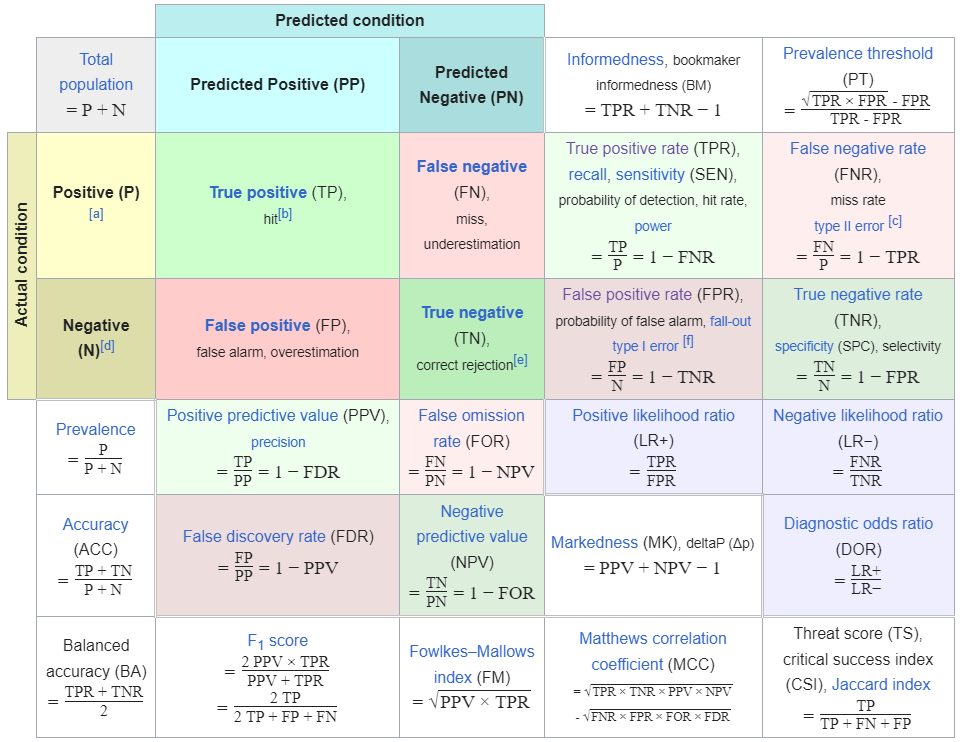
\includegraphics[width=0.9\textwidth]{figs/confmat.png}
    \label{fig:confusionMatrix}
    \caption{Macierz pomyłek oraz możliwe metryki oceny jakości klasyfikatora. Źródło:
    \href{https://en.wikipedia.org/wiki/Confusion_matrix}{en.wikipedia.org/wiki/Confusion\_matrix}}
\end{figure}

Wartość precision określa jak pewny jest klasyfikator przy wykrywaniu klasy pozytywnej, natomiast
recall mówi o tym jak dobrze klasyfikator \enquote{wyławia} przykłady pozytywne. Zauważmy jednak, iż
nie możemy stosować żadnej z tych metryk w odosobnieniu. Istotnie klasyfikator, który zwraca zawsze
klasę pozytywną ma maksymalny recall, a klasyfikator, który zwraca zawsze klasę negatywną ma
nieokreślony precision (i jest oczywiście beznadziejnym klasyfikatorem). Musimy więc zawsze
ewaluować model na obu tych metrykach i jedynie dobry wynik obu z nich mówi o jakości klasyfikatora.
Oczywiście czasami chcielibyśmy określić jakość modelu za pomocą jednej liczby, a niekoniecznie
sprawdzać zawsze macierz pomyłek (choć jest to bardzo użyteczne) lub podawać wartości dwóch metryk.
Metryką, która łączy precision i recall jest \emph{\(F_\beta\)--score} zdefiniowany jako
\[
F_\beta := (1 + \beta^2) \frac{\mathrm{Precision} \cdot \mathrm{Recall}}{\beta^2 \cdot \mathrm{Precision} + \mathrm{Recall}}\,, 
\]
gdzie \(\beta\) określa ile razy bardziej ważny jest recall od precision. Typowo używa się
\(F_1\)--score
\[
F_1 = 2\frac{\mathrm{Precision} \cdot \mathrm{Recall}}{\mathrm{Precision} + \mathrm{Recall}}\,. 
\]

Wiele klasyfikatorów oprócz twardych predykcji zwraca również rozkład prawdopodobieństwa nad
klasami. W przypadku klasyfikacji binarnej jest to oczywiście rozkład zero-jedynkowy z parametrem
\(p\) określającym prawdopodobieństwo klasy pozytywnej dla danego wektora cech. Standardowo
oczywiście twardą predykcją jest ta z klas, która ma większe prawdopodobieństwo, czyli (co
równoważne) predykcją jest klasa pozytywna jeśli \(p > 0.5\). W niektórych problemach chcemy jednak
zmienić ten próg i dokonać tzw. \textit{threshold tuning}. Wykresem, który pozwala na dokonanie
tuningu progu jest \emph{krzywa ROC} (z ang. \textit{Receiver Operatic Characteristic curve}), która
jest krzywą parametryczną wyznaczoną przez punkty \((\mathrm{FPR}(\mathrm{threshold}),
\mathrm{TPR}(\mathrm{threshold}))\) dla progów z zakresu \([0;1]\), gdzie
\[
\mathrm{TPR} := \frac{\mathrm{TP}}{\mathrm{TP + FN}}\,,\quad \mathrm{FPR} := \frac{\mathrm{FP}}{\mathrm{FP + TN}}\,.
\]
Metryką niezależną od wybranego progu jest tzw. \emph{AUROC} (z ang. \textit{Area under ROC curve})
zdefiniowany jako pole powierzchni pod krzywą ROC dla danego klasyfikatora. Zauważmy, że
klasyfikator losowy, który zwraca zawsze klasę pozytywną z prawdopodobieństwem równym wartości progu
ma wartość AUROC równą 0.5, natomiast idealny klasyfikator, który niezależnie od wartości progu
klasyfikuje wszystkie przykłady poprawnie ma AUROC równy 1.

Inną analogiczną metryką jest \emph{AUPRC}, gdzie zamiast krzywej ROC stosujemy krzywą \emph{PRC} (z
ang. \textit{Precision--Recall Curve}), w której zamiast TPR i FPR używamy odpowiednio Precision i
Recall. Metryka AUPRC jest często wykorzystywana w przypadku klasyfikacji ekstremalnie
niezbalansowanej, w której mamy bardzo mało (< 1\%) klasy pozytywnej.

W przypadku klasyfikacji wieloklasowej używamy zasadniczo takich samych metryk jak w klasyfikacji
binarnej, ale wprowadzamy mikro i makro uśrednianie (z ang. \textit{micro/macro-averaging}). Przez
\(\mathrm{TP}_k\) będziemy rozumieć liczbę prawidłowo zaklasyfikowanych przykładów z klasy \(k\),
\(\mathrm{FP}_k\) to liczba przykładów z innych klas, które zaklasyfikowaliśmy nieprawidłowo jako
\(k\)--tą klasę, \(\mathrm{FN}_k\) to liczba przykładów z klasy \(k\), które zaklasyfikowaliśmy jako
inną klasę. Wówczas odpowiednie metryki mają postać
\[
\begin{split}
&\mathrm{MicroPrecision} := \frac{\sum_{k} \mathrm{TP}_k}{\sum_{k} \mathrm{TP}_k + \sum_{k} \mathrm{FP}_k}\,,\\
&\mathrm{MacroPrecision} := \frac{1}{K} \sum_{k=1}^K \frac{\mathrm{TP}_k}{\mathrm{TP}_k + \mathrm{FP}_k}
\end{split}
\]
oraz
\[
\begin{split}
&\mathrm{MicroRecall} := \frac{\sum_{k} \mathrm{TP}_k}{\sum_{k} \mathrm{TP}_k + \sum_{k} \mathrm{FN}_k}\,,\\
&\mathrm{MacroRecall} := \frac{1}{K} \sum_{k=1}^K \frac{\mathrm{TP}_k}{\mathrm{TP}_k + \mathrm{FN}_k}\,.
\end{split}
\]
W przypadku klasyfikacji wieloklasowej macierz pomyłek jest macierzą wymiaru \(K \times K\), gdzie
\(K\) jest liczbą klas.


\subsubsection{Tuning hiperparametrów i walidacja skrośna}

Praktycznie wszystkie modele uczenia maszynowego mają hiperparametry, często liczne, które w
zauważalny sposób wpływają na wyniki, a szczególnie na underfitting i overfitting. Ich wartości
trzeba dobrać zatem dość dokładnie. Proces doboru hiperparametrów nazywa się tuningiem
hiperparametrów (z ang. \textit{hyperparameter tuning}).

Istnieje na to wiele sposobów. Większość z nich polega na tym, że trenuje się za każdym razem model
z nowym zestawem hiperparametrów i wybiera się ten zestaw, który pozwala uzyskać najlepsze wyniki.
Metody głównie różnią się między sobą sposobem doboru kandydujących zestawów hiperparametrów.
Najprostsze i najpopularniejsze to:
\begin{itemize}
\item pełne przeszukiwanie (z ang. \textit{grid search}) -- definiujemy możliwe wartości dla różnych
hiperparametrów, a metoda sprawdza ich wszystkie możliwe kombinacje (czyli siatkę),

\item losowe przeszukiwanie (z ang. \textit{randomized search}) -- definiujemy możliwe wartości jak
w pełnym przeszukiwaniu, ale sprawdzamy tylko ograniczoną liczbę losowo wybranych kombinacji.
\end{itemize}

Jak ocenić, jak dobry jest jakiś zestaw hiperparametrów? Nie możemy sprawdzić tego na zbiorze
treningowym -- wyniki byłyby zbyt optymistyczne. Nie możemy wykorzystać zbioru testowego --
mielibyśmy wyciek danych, bo wybieralibyśmy model explicite pod nasz zbiór testowy. Trzeba zatem
osobnego zbioru, na którym będziemy na bieżąco sprawdzać jakość modeli dla różnych hiperparametrów.
Jest to zbiór walidacyjny (z ang. \textit{validation set}). Zbiór taki wycina się ze zbioru
treningowego.

Jednorazowy podział zbioru na części nazywa się \textit{split validation} lub \textit{holdout}.
Używamy go, gdy mamy sporo danych, i 10-20\% zbioru jako dane walidacyjne czy testowe to dość dużo,
żeby mieć przyzwoite oszacowanie. Zbyt mały zbiór walidacyjny czy testowy da nam mało wiarygodne
wyniki -- nie da się nawet powiedzieć, czy zbyt pesymistyczne, czy optymistyczne. W praktyce
niestety często mamy mało danych. Trzeba zatem jakiejś magicznej metody, która stworzy nam więcej
zbiorów walidacyjnych z tej samej ilości danych. Taką metodą jest walidacja skrośna (z ang.
\textit{cross validation}, CV). Polega na tym, że dzielimy zbiór treningowy na \(K\) równych
podzbiorów, tzw. foldów. Każdy podzbiór po kolei staje się zbiorem walidacyjnym, a pozostałe łączymy
w zbiór treningowy. Trenujemy zatem \(K\) modeli dla tego samego zestawu hiperparametrów i każdy
testujemy na zbiorze walidacyjnym. Mamy \(K\) wyników dla zbiorów walidacyjnych, które możemy
uśrednić (i ewentualnie obliczyć odchylenie standardowe). Takie wyniki są znacznie bardziej
wiarygodne.


\section{Probabilistyka}

\subsection{Zmienne losowe}

Zmienna losowa to formalnie odwzorowanie ze zbioru zdarzeń elementarnych \(\Omega\) tj. zbioru
atomowych wyników doświadczenia losowego w zbiór \(\mathbb{R}^n\)
\[
\bm{X} : \Omega \mapsto \mathbb{R}^n\,.
\]
Jest to zatem funkcja, która przyporządkowuje zdarzeniom losowym wartość liczbową. Każda zmienna
losowa opisuje więc zmienną w klasycznym sensie, której wartości pochodzi z pewnego rozkładu.
Rozkład ten jest zadany jednoznacznie przez funkcję \(F: \mathbb{R}^n \mapsto [0;1]\) taką, że
\[
F(\bm{x}) := \Pr(\bm{X}^1 \leq \bm{x}^1, \ldots, \bm{X}^n \leq \bm{x}^n)\,,
\]
którą nazywa się dystrybuantą (z ang. \textit{cumulative distribution function, cdf}). Każdy rozkład
zmiennej losowej można opisać za pomocą dystrybuanty jednak jest to niewygodne. W dwóch przypadkach:
rozkładów dyskretnych i rozkładów ciągłych rozkład zmiennej losowej można opisać prościej za pomocą
odpowiednio funkcji prawdopodobieństwa (z ang. \textit{probability mass function, pmf}) oraz
gęstości prawdopodobieństwa (z ang. \textit{probability density function, pdf}).

\begin{definition}
Zmienna losowa \(\bm{X}\) ma dyskretny rozkład prawdopodobieństwa, jeśli istnieje skończony lub
przeliczalny zbiór \(\mc{S} \subset \mathbb{R}^n\) taki, że \(\Pr(\bm{X} \in \mc{S}) = 1\). Wówczas
rozkład ten jest zadany przez podanie funkcji prawdopodobieństwa \(p(\bm{x}) = \Pr(\bm{X} =
\bm{x})\) dla \(\bm{x} \in \mc{S}\).
\end{definition}

\begin{definition}
Zmienna losowa \(\bm{X}\) ma z kolei ciągły rozkład prawdopodobieństwa, jeśli istnieje funkcja \(p:
\mathbb{R}^n \mapsto \mathbb{R}_+\) taka, że
\[
\Pr(\bm{X}^1 \in (a_1;b_1), \ldots, \bm{X}^n \in (a_n;b_n)) = \int\limits_{a_1}^{b_1}\cdots\int\limits_{a_n}^{b_n} p(\bm{x}) \dd[n]{\bm{x}}
\]
dla dowolnej kostki \((a_1;b_1)\times\ldots\times(a_n;b_n)\).
\end{definition}

\begin{definition}[Wartości oczekiwanej]
Wartością oczekiwaną funkcji zmiennej losowej \(\bm{f}(\bm{X})\) nazywamy wektor
\(\mathbb{E}[\bm{f}(\bm{x})]\) określoną wzorem
\[
 \sum_{\bm{x} \in \mc{S}} \bm{f}(\bm{x}) p(\bm{x})\,,\quad \int\limits_{\mathbb{R}^n} \bm{f}(\bm{x}) p(\bm{x}) \dd[n]{\bm{x}}
\]
odpowiednio dla rozkładu dyskretnego i ciągłego.
\end{definition}

\begin{definition}[Macierzy kowariancji]
Macierzą kowariancji funkcji zmiennej losowej \(\bm{f}(\bm{X})\) nazywamy macierz
\[
\mathbb{E}\left[(\bm{f}(\bm{x}) - \bm{m_f})(\bm{f}(\bm{x}) - \bm{m_f})^T\right]\,,
\]
gdzie
\[
\bm{m_f} = \mathbb{E}\left[\bm{f}(\bm{x})\right]\,.
\]
Elementy diagonalne macierzy kowariancji nazywamy wariancjami, a elementy pozadiagonalne
kowariancjami.
\end{definition}

\begin{definition}[Kwantyla i mody]
Kwantylem \(q_p\) rzędu \(p \in (0;1)\) zmiennej losowej jednowymiarowej o rozkładzie ciągłym z
dystrybuantą \(F\) nazywamy dowolne rozwiązanie równania
\[
F(x) = p\,.
\]
Modą tej zmiennej nazywamy dowolne maksimum lokalne gęstości tego rozkładu.
\end{definition}

\begin{theorem}
Niech zmienna \(n\)--wymiarowa \(\bm{X}\) ma rozkład ciągły o gęstości \(p_{\bm{X}}\) i niech
\(\bm{Y}^i = \bm{\varphi}^i(\bm{X})\) dla \(i=1,\ldots,n\). Jeśli odwzorowanie \(\bm{\varphi}\) jest
różniczkowalne i odwracalne, przy czym odwzorowanie odwrotne \(\bm{\psi} = \bm{\varphi}^{-1}\) jest
różniczkowalne, to \(n\)--wymiarowa zmienna \(\bm{Y}\) ma rozkład o gęstości
\[
p_{\bm{Y}}(\bm{y}) = |J| p_{\bm{X}}(\bm{\psi}(\bm{y}))\,,
\]
gdzie \(J := \det \left[\pdv{\bm{\psi}^j}{\bm{y}^i}\right]\) jest jakobianem odwzorowania
\(\bm{\psi}\).
\end{theorem}

\begin{theorem}
Dla dowolnych zmiennych losowych \(\bm{X}\), \(\bm{Y}\) zachodzi
\[
p_{\bm{X}} (\bm{x}) = \int\limits_{\mathbb{R}^k} p(\bm{x}, \bm{y}) \dd[k]{\bm{y}}\quad\text{(sum rule)}
\]
\end{theorem}

\begin{theorem}
Dla dowolnych zmiennych losowych \(\bm{X}\), \(\bm{Y}\) zachodzi
\[
p(\bm{x}, \bm{y}) = p(\bm{x} \mid \bm{y}) p_{\bm{Y}}(\bm{y})\quad\text{(product rule)}
\]
\end{theorem}

\begin{theorem}
Zmienne losowe \(\bm{X}\) i \(\bm{Y}\) są niezależne wtedy i tylko wtedy, gdy
\[
p(\bm{x}, \bm{y}) = p_{\bm{X}}(\bm{x}) p_{\bm{Y}}(\bm{y})\quad\text{(independence)}
\]    
\end{theorem}

\begin{theorem}
Dla dowolnych zmiennych losowych \(\bm{X}\), \(\bm{Y}\) zachodzi    
\[
\underbrace{p(\bm{x} \mid \bm{y})}_\text{posterior} = \frac{\underbrace{p(\bm{y} \mid \bm{x})}_\text{likelihood} \underbrace{p_{\bm{X}}(\bm{x})}_\text{prior}}{ \underbrace{\int\limits_{\mathbb{R}^k} p(\bm{y} \mid \bm{x}) p_{\bm{X}}(\bm{x}) \dd[k]{\bm{x}}}_\text{evidence} }\quad\text{(Bayes theorem)}
\]    
\end{theorem}

\begin{definition}[Warunkowej wartości oczekiwanej]
Warunkową wartość oczekiwaną \(\bm{f}(\bm{X})\) pod warunkiem \(\bm{Y} = \bm{y}\) nazywamy wielkość
\[
\mathbb{E}[\bm{f}(\bm{x}) \mid \bm{y}] = \int\limits_{\mathbb{R}^n} \bm{f}(\bm{x}) p(\bm{x} \mid \bm{y}) \dd[n]{\bm{x}}
\]
\end{definition}


\subsection{Ważne rozkłady jednowymiarowe}

\begin{definition}[Rozkładu dwupunktowego]
Jeśli \(X\) jest zmienną losową rzeczywistą o rozkładzie dyskretnym i \(\mc{S} = \{x_1, x_2\}\) oraz
\(p(x_1) = p\), to mówimy, że \(X\) ma rozkład dwupunktowy z parametrem \(p\). Jeśli \(x_1 = 1\) i
\(x_2 = 0\) to taki rozkład dwupunktowy nazywamy \emph{rozkładem zero--jedynkowym} (lub rozkładem
Bernoulliego) i oznaczamy jako \(X \sim \mathrm{Ber}(p)\).
\end{definition}

\begin{definition}[Schematu dwumianowego]
Rozważmy doświadczenie losowe o dwu możliwych wynikach: sukces osiągamy z prawdopodobieństwem \(p\),
porażkę z prawdopodobieństwem \(1-p\). Doświadczenie tego rodzaju nazywamy \emph{próbą
Bernoulliego}. Doświadczenie takie jest modelowane zmienną losową o rozkładzie dwupunktowym z
parametrem \(p\). Schematem dwumianowym (lub schematem Bernoulliego) nazywamy doświadczenie
polegające na \(n\)--krotnym powtórzeniu próby Bernoulliego, przy założeniu, iż poszczególne próby
są od siebie niezależne.
\end{definition}

\begin{definition}[Rozkładu dwumianowego]
Niech \(X\) będzie zmienną losową taką, że \(X\) jest liczbą sukcesów w schemacie dwumianowym
długości \(n\) z prawdopodobieństwem sukcesu w każdej próbie równym \(p\). Wówczas
\[
\Pr(X = k) = {n \choose k} p^k (1 - p)^{n-k}\,.
\]
Rozkład prawdopodobieństwa określony powyższym wzorem nazywam się rozkładem dwumianowym o
parametrach \(n,p\). Jeśli zmienna \(X\) ma rozkład dwumianowy to stosujemy notację \(X \sim
\mathrm{Bin}(n,p)\).
\end{definition}

\begin{definition}[Rozkładu geometrycznego]
Mówimy, że zmienna losowa \(X\) ma rozkład geometryczny z parametrem \(p \in (0;1)\), tj. \(X \sim
\mathrm{Geo}(p)\), jeśli \(\mc{S} = \mathbb{N} \setminus \{0\}\), a funkcja prawdopodobieństwa ma
postać
\[
p(x) = (1-p)^{x-1}p\,.
\]
Zmienna \(X\) opisuje czas oczekiwania na pierwszy sukces w schemacie dwumianowym o nieskończonej
długości.
\end{definition}

\begin{definition}[Rozkładu Poissona]
Jeśli zmienna \(X\) o wartościach w \(\mathbb{N}\) opisuje liczbę wystąpień pewnego powtarzalnego
zdarzenia w przedziale czasowym \([0;t]\), przy czym spełnione są następujące założenia:
\begin{itemize}
\item powtórzenia zdarzenia występują niezależnie od siebie;    
\item \enquote{intensywność} wystąpień \(r\) jest stała;
\item w danej chwili (rozumianej jako odpowiednio mały przedział) może zajść co najwyżej jedno
zdarzenie
\end{itemize}

to zmienna ta ma rozkład Poissona z parametrem \(\lambda = rt\), tj. \(X \sim
\mathrm{Pos}(\lambda)\). Jeśli \(X \sim \mathrm{Pos}(\lambda)\), to
\[
\Pr(X = k) = \frac{\e^{-\lambda} \lambda^k}{k!}\,.
\]
\end{definition}

\begin{theorem}[Poissona]
Niech \((X_n)\) będzie ciągiem zmiennych losowych takich, że \(X_n \sim \mathrm{Bin}(n, p_n)\),
gdzie \((p_n)\) jest ciągiem takim, że
\[
\lim_{n \to \infty} n p_n = \lambda
\]
dla pewnej liczby \(\lambda > 0\). Wówczas
\[
\lim_{n \to \infty} \Pr(X_n = k) = \frac{\e^{-\lambda} \lambda^k}{k!}\,.
\]
\end{theorem}

\begin{definition}[Rozkładu jednostajnego]
Mówimy, że zmienna \(X\) o rozkładzie ciągłym ma rozkład jednostajny na przedziale \([a;b]\) tzn.
\(X \sim \mc{U}(a,b)\) jeśli jej gęstość wyraża się wzorem
\[
p(x) = \begin{cases}
    \frac{1}{b - a}\,, &x\in[a;b]\\
    0\,,&x\notin[a;b]
\end{cases}\quad.
\]
\end{definition}

\begin{definition}[Rozkładu wykładniczego]
Niech \(T\) będzie zmienną modelującą czas oczekiwania na pierwsze zdarzenie w ciągu zdarzeń takim,
że czas wystąpienia każdego z nich w przedziale \([0;t]\) jest opisany przez zmienną \(X \sim
\mathrm{Pos}(\lambda t)\). wtedy
\[
\Pr(T > t) = \Pr(X = 0) = \e^{-\lambda t}
\]
oraz
\[
\Pr(T > 0) = 1\,.
\]
Mówimy wtedy, że \(T\) ma rozkład wykładniczy z parametrem \(\lambda\), tzn. \(T \sim
\mathrm{Exp}(\lambda)\). Gęstość rozkładu wykładniczego ma postać
\[
p(t) = \begin{cases}
    0\,,&t \leq 0\\
    \lambda \e^{-\lambda t}\,,&t > 0
\end{cases}\quad.
\]
\end{definition}

\begin{definition}[Rozkładu normalnego]
Mówimy, że zmienna losowa \(X\) o gęstości \(p(x)\) ma rozkład normalny z parametrami \(\mu \in
\mathbb{R} , \sigma^2 \in [0;+\infty)\), tzn. \(X \sim \mc{N}(\mu,\sigma^2)\), jeśli    
\[
p(x) = \frac{1}{\sigma\sqrt{2 \pi}} \exp\left(-\frac{(x-\mu)^2}{2\sigma^2}\right)\,.
\]
Jeśli \(\mu=0\) i \(\sigma=1\), to taki rozkład nazywamy standardowym rozkładem normalnym.
\end{definition}


\subsection{Wielowymiarowy rozkład normalny}

\begin{definition}[Standardowego wielowymiarowego rozkładu normalnego]
Zmienna losowa \(\bm{X}\) ma standardowy \(n\)--wymiarowy rozkład normalny jeśli jej składowe są
niezależne i dla każdego \(i=1,\ldots,n\) \(\bm{X}^i \sim \mc{N}(0,1)\). Jest to rozkład ciągły o
gęstości
\[
p(\bm{x}) = \frac{1}{\sqrt{(2\pi)^n}}\exp\left(-\frac{1}{2}\bm{x}^T\bm{x}\right)\,.
\]
\end{definition}

\begin{definition}[Wielowymiarowego rozkładu normalnego]
Zmienna losowa \(\bm{X}\) ma \(n\)--wymiarowy rozkład normalny (z ang. \textit{Multivariate Normal
Distribution, MVN}), tzn. \(\bm{X} \sim \mc{N}(\bm{\mu}, \bm{\Sigma})\) jeśli istnieje
\(k\)--wymiarowa zmienna losowa \(\bm{Z}\) o standardowym rozkładzie normalnym dla pewnego \(k \leq
n\) oraz istnieje \(\bm{\mu} \in \mathbb{R}^n\) i macierz \(\bm{A} \in \mathbb{R}^{n \times k}\)
takie, że \(\bm{\Sigma} = \bm{A}\bm{A}^T\) oraz
\[
\bm{X} = \bm{A}\bm{Z} + \bm{\mu}\,.
\]
Jeśli macierz \(\bm{\Sigma}\) jest dodatnio określona, to rozkład \(\mc{N}(\bm{\mu}, \bm{\Sigma})\)
jest ciągły, a jego gęstość jest dana przez
\[
p(\bm{x}) = \frac{1}{\sqrt{(2\pi)^n\det\bm{\Sigma}}}\exp\left(-\frac{1}{2}(\bm{x}-\bm{\mu})^T\bm{\Sigma}^{-1}(\bm{x}-\bm{\mu})\right)
\]
Macierz \(\bm{\Sigma}^{-1}\) nazywa się \emph{macierzą precyzji}.
\end{definition}

Poziomice gęstości niezdegenerowanego wielowymiarowego rozkładu normalnego są elipsoidami, których
półosie są skierowane wzdłuż wektorów własnych macierzy \(\bm{\Sigma}\) i mają długości
proporcjonalne do pierwiastka z wartości własnych.

\begin{theorem}[Własności niezdegenerowanego rozkładu normalnego]\label{th:mvn} Niech \(\bm{X} \sim
\mc{N}(\bm{\mu}, \bm{\Sigma})\) dla dodatnio określonej macierzy \(\bm{\Sigma}\), wówczas
\begin{enumerate}
\item Wszystkie rozkłady brzegowe i warunkowe \(\bm{X}\) są rozkładami normalnymi. Istotnie jeśli
\[
\mqty[\bm{x} \\ \bm{y}] \sim \mathcal{N}\left(\mqty[\bm{\mu}_{\bm{x}} \\ \bm{\mu}_{\bm{y}}], \mqty[\bm{\Sigma}_{\bm{xx}} & \bm{\Sigma}_{\bm{xy}} \\ \bm{\Sigma}_{\bm{yx}} & \bm{\Sigma}_{\bm{yy}}] \right)
\]
to można pokazać, iż
\[
\bm{x} \sim \mathcal{N}(\bm{\mu}_{\bm{x}}, \bm{\Sigma}_{\bm{xx}})\,,\quad \bm{y} \sim \mathcal{N}(\bm{\mu}_{\bm{y}}, \bm{\Sigma}_{\bm{yy}})\,.
\]
oraz \(\bm{x} \mid \bm{y} \sim \mathcal{N}(\bm{\mu}_{\bm{x}\mid\bm{y}},
\bm{\Sigma}_{\bm{x}\mid\bm{y}})\), gdzie
\[
\bm{\mu}_{\bm{x}\mid\bm{y}} = \bm{\mu}_{\bm{x}} + \bm{\Sigma}_{\bm{xy}}\bm{\Sigma}_{\bm{yy}}^{-1}(\bm{y} - \bm{\mu}_{\bm{y}})\,,\quad \bm{\Sigma}_{\bm{x}\mid\bm{y}} = \bm{\Sigma}_{\bm{xx}} - \bm{\Sigma}_{\bm{xy}}\bm{\Sigma}_{\bm{yy}}^{-1}\bm{\Sigma}_{\bm{yx}}\,.
\]

\item Zmienne składowe \(\bm{X}^1,\ldots,\bm{X}^n\) są niezależne wtedy i tylko wtedy, gdy
\(\bm{\Sigma}\) jest macierzą diagonalną.
\end{enumerate}
\end{theorem}


\subsection{Wnioskowanie statystyczne}

Niech zmienna losowa \(\bm{X}\) określa model rozkładu pewnej cechy (cech) w ustalonym zbiorze
instancji (tzw. \emph{populacji generalnej}). Innymi słowy, przyjmujemy, że wartości cech zachowują
się jakby zostały wybrane losowo zgodnie z rozkładem zmiennej \(\bm{X}\). Do podstawowych zagadnień
wnioskowania statystycznego należą:
\begin{itemize}
\item oszacowanie wielkości charakteryzujących rozkład \(\bm{X}\) (np. wartości średniej albo
wariancji);
\item weryfikacja hipotez dotyczących rozkładu \(\bm{X}\) (tym nie będziemy się zajmować).
\end{itemize}

\begin{definition}[Modelu statystycznego]
Modelem statystycznym nazywamy parę \((\mc{P}, \mc{X})\), gdzie \(\mc{P}\) jest rodziną rozkładów
prawdopodobieństwa na zbiorze \(\mc{X}\). Zazwyczaj przyjmuje się
\[
\mc{P} = \{p(\cdot \mid \bm{\theta}) : \bm{\theta} \in \Theta \} 
\]
dla pewnego zbioru parametrów \(\Theta\). Model statystyczny nazywamy \emph{parametrycznym} jeśli
\(\Theta \subset \mathbb{R}^k\).
\end{definition}

\begin{definition}[Prostej próby losowej]
Prostą próbą losową o liczności \(n\) nazywamy ciąg niezależnych zmiennych losowych
\(\bm{X}_1,\ldots,\bm{X}_n\) o tym samym rozkładzie \(p(\cdot \mid \bm{\theta}) \in \mc{P}\) (z ang.
\textit{independent and identically distributed, i.i.d}).
\end{definition}

\begin{definition}[Estymatora]
Estymatorem nazywa się statystykę \(\hat{\theta}(\bm{X}_1,\ldots,\bm{X}_n)\) służącą do oszacowania
wartości parametru \(\theta\). Liczbę \(\hat{\theta}(\bm{x}_1,\ldots,\bm{x}_n)\) dla konkretnej
realizacji prostej próby losowej nazywa się wartością estymatora albo estymatą.
\end{definition}

\begin{definition}[Funkcji wiarygodności]
Funkcją wiarygodności (z ang. \textit{likelihood function}) dla modelu \(\mc{P} = \{p(\cdot \mid \bm{\theta}) :
\bm{\theta} \in \Theta\}\) nazywamy funkcję
\[
\mc{L}: \mathbb{R}^n \times \Theta \ni (\bm{x},\bm{\theta}) \mapsto \mc{L}(\bm{x};\bm{\theta}) \in [0; +\infty)
\]
wyznaczającą rozkład łączny obserwowanych danych jako funkcję parametru \(\bm{\theta}\).    
\end{definition}

Niech \(\bm{X}_1,\ldots,\bm{X}_n\) będzie prostą próbą losową. Jeśli \(p(\cdot \mid \bm{\theta})\)
opisuje rozkład warunkowy, z którego pochodzą obserwacje, to
\[
\mc{L}(\bm{x}_1,\ldots,\bm{x}_n;\bm{\theta}) = \prod_{i=1}^n p(\bm{x}_i \mid \bm{\theta})\,.
\]
Dla wygody obliczeń często rozważa się tzw. zanegowaną logarytmiczną funkcję wiarygodności (z ang.
\textit{Negated Log-Likelihood function, NLL}), tzn.
\[
L(\bm{x};\bm{\theta}) = - \log \mc{L}(\bm{x};\bm{\theta})\,.
\]
Wówczas dla realizacji prostej próby losowej mamy
\[
L(\bm{x}_1,\ldots,\bm{x}_n;\bm{\theta}) = -\sum_{i=1}^n \log p(\bm{x}_i \mid \bm{\theta})\,.
\]

\begin{definition}[Estymatora największej wiarygodności]
Estymatorem największej wiarygodności (z ang. \textit{Maximum Likelihood Estimator, MLE}) nazywamy
funkcję \(\bm{\hat{\theta}}\), która przy ustalonych wartościach obserwacji (realizacji prostej
próby losowej) \(\{\bm{x}_1,\ldots,\bm{x}_n\}\) maksymalizuje wartość funkcji wiarygodności lub, co
równoważne, minimalizuje wartość zanegowanej logarytmicznej funkcji wiarygodności tj.
\[
\bm{\hat \theta}(\bm{x}_1,\ldots,\bm{x}_n) = \arg \min_{\bm{\theta} \in \Theta} \left[- \sum_{i=1}^n \log p(\bm{x}_i \mid \bm{\theta})\right]\,.
\]
\end{definition}
    
Jeśli funkcja wiarygodności jest różniczkowalna względem \(\bm{\theta}\) dla dowolnych \(\bm{x}^i\),
to MLE można czasem wyznaczyć analitycznie korzystając z warunku koniecznego optymalności, tzn.
rozwiązując układ równań
\[
\pdv{L(\bm{x}_1,\ldots,\bm{x}_n; \bm{\theta})}{\bm{\theta}} = 0\,.
\]
Jeśli MLE nie da się wyliczyć analitycznie, wyznacza się je przy użyciu algorytmów optymalizacji
numerycznej. Estymatory MLE są asymptotycznie nieobciążone.

\begin{definition}[Estymatora MAP]
Estymatorem MAP (z ang. \textit{Maximum a Posteriori Estimator, MAP}) nazywamy funkcję
\(\bm{\hat\theta}\), która przy ustalonych wartościach obserwacji (realizacji prostej próby losowej)
\(\{\bm{x}_1,\ldots,\bm{x}_n\}\) maksymalizuje wartość iloczynu funkcji wiarygodności i priora nad
wartościami parametrów lub, co równoważne, minimalizuje zregularyzowaną logarytmiczną funkcję
wiarygodności tj.
\[
\bm{\hat\theta}(\bm{x}_1,\ldots,\bm{x}_n) = \arg \min_{\bm{\theta} \in \Theta} \left[ - \sum_{i=1}^n \log p(\bm{x}_i \mid \bm{\theta}) - n \log p(\bm{\theta}) \right]\,.
\]
\end{definition}


\subsection{Liczby losowe w komputerze}

Opiszemy jeszcze pokrótce metody generowania liczb pseudolosowych z dowolnych rozkładów
prawdopodobieństwa w sposób algorytmiczny. Podstawowym narzędziem, którego będziemy potrzebować do
generowania próbek z bardziej skomplikowanych rozkładów będzie prosty generator liczb z rozkładu
jednostajnego \(\mc{U}(0,1)\). Moglibyśmy oczywiście wykorzystać jakieś fizyczne urządzenie lub
proces, który generuje liczby prawdziwie losowe (np. detektor Geigera-Mullera, szum lamp
elektronowych, ruletka), ale błędem byłaby rezygnacja z odtwarzalności. Poszukujemy zatem
deterministycznej metody, która generuje sekwencje liczb, które są w przybliżeniu losowe. Podstawową
metodą do algorytmicznego generowania liczb pseudolosowych jest tzw. \emph{liniowy generator
kongruentny} (z ang. \textit{Linear Congruential Generator, LCG}), który jest opisany zależnością
rekurencyjną
\[
I_{j+1} = (a I_j + c) \mod m\,,
\]
gdzie \(a, c, m\) to pewne ustalone dodatnie liczby całkowite, a \(I_0\) to tzw. ziarno (z ang.
\textit{seed}). LCG generuje liczby całkowite, więc w dużym uproszczeniu liczby zmiennoprzecinkowe z
rozkładu \(\mc{U}(0,1)\) otrzymujemy jako \(I_j / m\) (trzeba tutaj jednak uwzględnić problemy
wynikające z arytmetyki zmiennoprzecinkowej).

Mając już generator liczb z rozkładu jednostajnego \(\mc{U}(0,1)\) i znając jawny wzór na
dystrybuantę \(F(x)\) innego rozkładu jednowymiarowego \(\mc{D}\) możemy generować liczby z tego
rozkładu korzystając z tzw. \emph{metody odwrotnej dystrybuanty}. Istotnie, jeśli \(U \sim
\mc{U}(0,1)\), to \(F^{-1}(U) \sim \mc{D}\). Istotnie
\[
\Pr(F^{-1}(U) \leq x) = \Pr(U \leq F(x)) = F(x)\,.
\]
Metoda ta ma jedną zasadniczą wadę -- musimy znać jawny wzór na dystrybuantę \(F(x)\). W przypadku
np. tak ważnych rozkładów, jak rozkład normalny dystrybuanta nie jest funkcją elementarną i metoda
ta nie jest najlepsza. W przypadku rozkładu normalnego znacznie lepszą metodą jest tzw. \emph{metoda
Boxa--Mullera}. Weźmy rozkład łączny dwóch niezależnych zmiennych losowych \(X, Y\) pochodzących ze
standardowego rozkładu normalnego
\[
p(x, y) = \frac{1}{2\pi}\exp(\frac{1}{2}(x^2 + y^2))\,.
\]
Skorzystamy ze wzoru na transformację zmiennych losowych. Istotnie niech
\[
X = \sqrt{Z} \cos \Phi\,,\quad Y = \sqrt{Z} \sin \Phi\,,
\]
dla \(0 < Z\) oraz \( 0 \leq \Phi < 2\pi\), wówczas
\[
q(z, \phi) = p(x(z,\phi), y(z,\phi)) \mqty| \frac{1}{2\sqrt{z}}\cos\phi & \frac{1}{2\sqrt{z}}\sin\phi \\ -\sqrt{z}\sin\phi & \sqrt{z}\cos\phi| = \frac{1}{4\pi}\e^\frac{z}{2}\,.
\]
Zauważmy, że otrzymaliśmy sferycznie symetryczny rozkład wykładniczy. Możemy zatem wylosować z
rozkładu jednostajnego kąt \(\phi\) oraz z rozkładu wykładniczego wartość \(z\) korzystając z metody
odwrotnej dystrybuanty. Wówczas wartości \(x = \sqrt{z}\cos\phi\), \(y = \sqrt{z}\sin\phi\) będą
pochodzić ze standardowego rozkładu normalnego. Aby wygenerować próbki z ogólnego wielowymiarowego
rozkładu normalnego, korzystamy z definicji, tj. najpierw generujemy \(n\) próbek ze standardowego
rozkładu normalnego, a następnie korzystamy z przekształcenia afinicznego \(\bm{x} = \bm{A}\bm{z} +
\bm{\mu}\), gdzie \(\bm{\Sigma} = \bm{A}\bm{A}^T\).


\subsection{Monte Carlo}

Umiemy już generować próbki z wielowymiarowego rozkładu normalnego. Chcemy teraz poznać metodę,
która umożliwi generowanie próbek ze skomplikowanych, wielowymiarowych rozkładów prawdopodobieństwa,
których gęstość znamy jedynie z dokładnością do stałej normalizującej, tj. znamy jedynie
\(\tilde{p}(\bm{x}) = Z p(\bm{x})\). Ograniczenie to wynika z chęci próbkowania z posteriora
\(p(\bm{x} \mid \bm{y})\) w sytuacji, gdy znamy jedynie rozkład łączny \(p(\bm{x}, \bm{y}) =
p(\bm{y} \mid \bm{x}) p_{\bm{X}}(\bm{x})\). Okazuje się, iż znajomość rozkładu jedynie z
dokładnością do stałej normalizującej jest wystarczająca do generowania próbek z tego rozkładu.
Generowanie próbek z kolei wystarcza natomiast, na mocy silnego prawa wielkich liczb, do szacowania
wartości średnich dowolnych funkcji zmiennej \(\bm{x}\). Przypomnijmy, iż na mocy silnego prawa
wielkich liczb ciąg średnich częściowych \((\overline{\bm{X}}_n)\) ciągu zmiennych losowych
\((\bm{X}_n)\) i.i.d. z rozkładu \(\bm{X} \sim \mathcal{D}\) jest zbieżny z prawdopodobieństwem 1 do
wartości oczekiwanej \(\mathbb{E}[\bm{X}]\) tj.
\[
\Pr\left(\lim_{n \to \infty} \overline{\bm{X}}_n = \mathbb{E}[\bm{X}]\right) = 1\,.
\]
Wartość oczekiwaną \(\mathbb{E}[\bm{X}]\) możemy zatem przybliżyć średnią \(\overline{\bm{X}}_n\) z
dużej ilości próbek.

Pozostaje pytanie w jaki sposób generować próbki ze skomplikowanych rozkładów prawdopodobieństwa,
których gęstości znamy jedynie z dokładnością do stałej normalizującej. Poniżej przedstawimy dwa
algorytmy próbkowania: algorytm IS oraz Metropolisa--Hastingsa będący szczególną realizacją całej
rodziny algorytmów próbkowania zwanych Markov Chain Monte Carlo (MCMC).


\subsubsection{Algorytm Importance Sampling}

Załóżmy, iż chcemy obliczyć wartość oczekiwaną pewnej funkcji zmiennej losowej \(\bm{x}\) względem
skomplikowanego rozkładu prawdopodobieństwa \(p(\bm{x})\), który znamy jedynie z dokładnością do
stałej normalizującej
\[
p(\bm{x}) = \frac{1}{Z_p}\tilde{p}(\bm{x})
\]
tj. szukamy
\[
\mathbb{E}_p[f(\bm{x})] = \int f(\bm{x}) p(\bm{x})\dd[n]\bm{x}\,.
\]
Jeśli umiemy generować próbki \(\bm{x}\) z innego (prostszego) rozkładu \(q(\bm{x})\) (np.
wielowymiarowego rozkładu normalnego), który nazywamy rozkładem proponującym kandydatów (z ang.
\textit{proposal distribution}) to możemy zapisać
\[
\begin{split}
\mathbb{E}_p[f(\bm{x})] &= \int\limits_{\mathbb{R}^n}f(\bm{x})p(\bm{x})\dd[n]\bm{x} = \int\limits_{\mathbb{R}^n}f(\bm{x})\frac{p(\bm{x})}{q(\bm{x})}q(\bm{x})\dd[n]\bm{x}\\
&=\mathbb{E}_q\left[f(\bm{x}) \frac{p(\bm{x})}{q(\bm{x})}\right] = \frac{Z_q}{Z_p}\mathbb{E}_q\left[f(\bm{x}) \frac{\tilde{p}(\bm{x})}{\tilde{q}(\bm{x})}\right]\,.
\end{split}
\]
Zakładamy tutaj, iż nośnik rozkładu \(p\) zawiera się w nośniku \(q\) tj. \(\text{supp}\,p \subseteq
\text{supp}\,q\). Stosunek stałych \(Z_p / Z_q\) również możemy oszacować z próbek z \(q\), gdyż
mamy
\[
Z_p = \int\limits_{\mathbb{R}^n}\tilde{p}(\bm{x})\dd[n]{\bm{x}} = Z_q\int\limits_{\mathbb{R}^n}\frac{\tilde{p}(\bm{x})}{\tilde{q}(\bm{x})} q(\bm{x})\dd[n]{\bm{x}} = Z_q \mathbb{E}_q\left[\frac{\tilde{p}(\bm{x})}{\tilde{q}(\bm{x})}\right]\,,
\]
skąd ostatecznie
\[
\mathbb{E}_p[f(\bm{x})] = \frac{\mathbb{E}_q\left[f(\bm{x}) \frac{\tilde{p}(\bm{x})}{\tilde{q}(\bm{x})}\right]}{\mathbb{E}_q\left[\frac{\tilde{p}(\bm{x})}{\tilde{q}(\bm{x})}\right]}\,.
\]
Jeśli z rozkładu \(q\) wygenerowaliśmy próbki \(X = \left\{\bm{x}_1,\ldots,\bm{x}_m\right\}\) to na
mocy silnego prawa wielkich liczb mamy
\[
\boxed{
\mathbb{E}_p[f(\bm{x})] \approx \frac{\sum_{i=1}^m f(\bm{x}_i) \frac{\tilde{p}(\bm{x}_i)}{\tilde{q}(\bm{x}_i)}}{\sum_{j=1}^m \frac{\tilde{p}(\bm{x}_j)}{\tilde{q}(\bm{x}_j)}} = \sum_{i=1}^m \lambda_i f(\bm{x}_i)\,,
}
\]
gdzie
\[
\boxed{
\lambda_i = \frac{\tilde{p}(\bm{x}_i) / \tilde{q}(\bm{x}_i)}{\sum_{j=1}^m \tilde{p}(\bm{x}_j) / \tilde{q}(\bm{x}_j) }\,.
}
\]
Algorytm Importance Sampling jest prostym algorytmem Monte Carlo, który ma jeden zasadniczy problem.
W jaki sposób mamy wybrać rozkład proponujący kandydatów \(q\)? Pewną odpowiedź na to pytanie
sugeruje analiza wariancji statystyki 
\[
\overline{f}_m(\bm{x}_1,\ldots,\bm{x}_m) = \frac{1}{m}\sum_{i=1}^m \frac{f(\bm{x}_i)p(\bm{x}_i)}{q(\bm{x}_i)}
\]
dla \(\bm{x}_i \sim q\) mamy
\[
\begin{split}
\mathbb{V}[\overline{f}_m] &= \frac{1}{m}\mathbb{V}_q\left[f(\bm{x})\frac{p(\bm{x})}{q(\bm{x})}\right] = \frac{1}{m}\int\limits_{\mathbb{R}^n}\frac{(f(\bm{x})p(\bm{x}) - \mu_fq(\bm{x}))^2}{q(\bm{x})}\dd[n]{\bm{x}}\,.
\end{split}
\]
Chcemy oczywiście, aby wariancja była jak najmniejsza, gdyż wówczas mała liczba próbek da dobre
przybliżenie wartości oczekiwanej. Rozkład proponujący kandydatów powinien być zatem proporcjonalny
do \(f(\bm{x})p(\bm{x})\), co może być trudne do praktycznego zrealizowania.


\subsubsection{Algorytm Metropolisa--Hastingsa}

Cała klasa algorytmów próbkowania MCMC opiera się na idei wyrażenia generowania próbek jako ewolucji
pewnego łańcucha Markowa.

\begin{definition}[Łańcucha Markowa]
Łańcuchem Markowa nazwiemy ciąg zmiennych losowych \((\bm{X}_t)\) o wartościach w \(\mathbb{R}^n\)
taki, że spełnione jest \emph{kryterium Markowa}
\[
\begin{split}
\forall A \subset \mathbb{R}^n :\, &\Pr(\bm{X}_t \in A \mid \bm{X}_{t-1} = \bm{x}_{t-1}, \ldots, \bm{X}_0 = \bm{x}_0) \\
&= \Pr(\bm{X}_t \in A \mid \bm{X}_{t-1} = \bm{x}_{t-1})\,.
\end{split}
\]
Elementy ciągu nazywamy stanami łańcucha.
\end{definition}

Dany łańcuch jest zadany jednoznacznie przez podanie gęstości prawdopodobieństwa przejścia łańcucha
ze stanu \(\bm{x} \to \bm{y}\), którą będziemy oznaczać przez \(\pi(\bm{y} \mid \bm{x})\)
(zakładamy, iż prawdopodobieństwo przejścia jest niezależne od chwili \(t\) -- łańcuch taki nazywamy
jednorodnym). Funkcja \(\pi\) spełnia oczywiście warunek unormowania
\[
\int\limits_{\mathbb{R}^n} \pi(\bm{y} \mid \bm{x}) \dd[n]{\bm{y}} = 1\,,
\]
istotnie prawdopodobieństwo przejścia gdziekolwiek ze stanu \(\bm{x}\) jest równe 1. Będziemy
zakładać dodatkowo, iż \(\forall \bm{x},\bm{y}\in\mathbb{R}^n: \pi(\bm{y} \mid \bm{x}) > 0\).
Rozkład \(p(\bm{x})\) łańcucha Markowa (tj. rozkład prawdopodobieństwa z którego losujemy stan
łańcucha w danej chwili \(t\)) z daną funkcją przejścia \(\pi\) nazwiemy rozkładem stacjonarnym tego
łańcucha jeśli
\[
p(\bm{y}) = \int\limits_{\mathbb{R}^n} \pi(\bm{y} \mid \bm{x})p(\bm{x}) \dd[n]{\bm{x}}\,.
\]
Rozkład stacjonarny danego łańcucha oznaczymy przez \(p^*(\bm{x})\). Zauważmy, iż jeśli stan
początkowy łańcucha \(\bm{X}_0\) pochodzi z rozkładu stacjonarnego \(p^*\) to każdy kolejny stan
\(\bm{X}_t\) również pochodzi z rozkładu stacjonarnego. Jeśli z kolei stan początkowy pochodzi z
jakiegoś innego rozkładu \(p_0\) to rozkład łańcucha w chwili \(t\) jest dany przez relację
rekurencyjną
\[
p_t(\bm{y}) = \int\limits_{\mathbb{R}^n} \pi(\bm{y} \mid \bm{x})p_{t-1}(\bm{x}) \dd[n]{\bm{x}}\,,\quad\text{dla \(t > 1\).}
\]
Rozkładem granicznym łańcucha Markowa nazwiemy granicę w sensie zbieżności punktowej
\[
\lim_{t\to\infty} p_t(\bm{x})\,.
\]
Przy podanych wyżej założeniach istnieje twierdzenie, które mówi iż taki łańcuch Markowa posiada
jednoznaczny rozkład stacjonarny tożsamy z rozkładem granicznym. Ponadto warunkiem wystarczającym,
aby dany rozkład \(p(\bm{x})\) był rozkładem stacjonarnym łańcucha Markowa jest
\[
\forall\bm{x}, \bm{y} \in \mathbb{R}^n: \pi(\bm{y}\mid\bm{x}) p(\bm{x}) = \pi(\bm{x} \mid \bm{y}) p(\bm{y})\,,
\]
co wynika z scałkowania powyższego równania
\[
\int\limits_{\mathbb{R}^n} \pi(\bm{y}\mid\bm{x}) p(\bm{x}) \dd[n]{\bm{x}} = \int\limits_{\mathbb{R}^n} \pi(\bm{x} \mid \bm{y}) p(\bm{y}) \dd[n]{\bm{x}} = p(\bm{y}) \int\limits_{\mathbb{R}^n} \pi(\bm{x} \mid \bm{y}) \dd[n]{\bm{x}} = p(\bm{y})\,.
\]
Kryterium to nazywamy \emph{kryterium lokalnego balansu} (z ang. \textit{detailed balance
condition}).

Podstawowa idea wykorzystania łańcuchów Markowa do generowania próbek ze skomplikowanego rozkładu
\(p\) jest więc następująca: tworzymy łańcuch Markowa, dla którego \(p\) jest rozkładem
stacjonarnym, wówczas rozpoczynając w dowolnym dopuszczalnym stanie początkowym \(\bm{X}_0\) po
wykonaniu dużej liczby kroków (etap ten nazywamy okresem przejściowym z ang. \textit{burn-in
period}) stan \(\bm{X}_t\) (dla \(t \gg 1\)) tego łańcucha będzie w przybliżeniu pochodził z
rozkładu granicznego \(p\) (nie jest jednak prosto stwierdzić po jak długim okresie przejściowym
przybliżenie to jest wystarczająco dobre). Aby otrzymać z takiej procedury próbki prawdziwie i.i.d.
każda z próbek musiałaby pochodzić z ponownego uruchomienia takiego łańcucha. Oczywiście jest to
nieefektywne, więc w praktyce generujemy próbki z jednego łańcucha po prostu odrzucając pewne z nich
tak aby uniknąć znaczących korelacji. Pozostaje pytanie jak skonstruować funkcję przejścia
\(\pi(\bm{y} \mid \bm{x})\) dla danego rozkładu granicznego \(p(\bm{x})\). Podstawową konstrukcję
podaje algorytm Metropolisa--Hastingsa.
\begin{tcolorbox}[title=Algorytm Metropolisa--Hastingsa, breakable, boxrule=0pt]
\begin{enumerate}
\item Jako stan początkowy przyjmij dowolną dopuszczalną wartość \(\bm{x}_0\).

\item Będąc w aktualnym stanie \(\bm{x}\) z prostego rozkładu proponującego kandydatów \(q(\bm{y}
\mid \bm{x})\) wylosuj kandydata \(\bm{y}\) na wartość łańcucha w kolejnym stanie.

\item Z prawdopodobieństwem
\[
r(\bm{y} \mid \bm{x}) = \min\left\{1, \frac{p(\bm{y})q(\bm{x} \mid \bm{y})}{p(\bm{x})q(\bm{y} \mid \bm{x})}\right\}
\]
zaakceptuj kandydata jako nowy stan i przejdź do stanu \(\bm{y}\). W przeciwnym razie pozostań w
stanie \(\bm{x}\).

\item GOTO 2.
\end{enumerate}
\end{tcolorbox}

Funkcja przejścia ma zatem postać
\[
\pi_\text{MH}(\bm{y}\mid\bm{x}) = q(\bm{y} \mid \bm{x}) r(\bm{y} \mid \bm{x})\,.
\]
Pozostaje tylko wykazać, iż spełnione jest kryterium lokalnego balansu. Istotnie mamy
\[
\begin{split}
&\pi_\text{MH}(\bm{y}\mid\bm{x})p(\bm{x}) = \min\left\{q(\bm{y}\mid\bm{x})p(\bm{x}), q(\bm{x}\mid\bm{y})p(\bm{y})\right\}\\
&\pi_\text{MH}(\bm{x}\mid\bm{y})p(\bm{y}) = \min\left\{q(\bm{x}\mid\bm{y})p(\bm{y}), q(\bm{y}\mid\bm{x})p(\bm{x})\right\}
\end{split}\quad,
\]
skąd \(\pi_\text{MH}(\bm{y}\mid\bm{x})p(\bm{x}) = \pi_\text{MH}(\bm{x}\mid\bm{y})p(\bm{y})\).
Zauważmy, iż nie musimy znać \(p(\bm{x})\) z dokładnością do stałej normalizującej, gdyż
\[
\frac{p(\bm{y})}{p(\bm{x})} = \frac{\tilde{p}(\bm{y})/Z_p}{\tilde{p}(\bm{x})/Z_p} = \frac{\tilde{p}(\bm{y})}{\tilde{p}(\bm{x})}\,.
\]
Poza algorytmem Metropolisa--Hastingsa jest wiele innych algorytmów z rodziny MCMC. Większość z nich
implementuje konkretny sposób generowania (zostawiając resztę struktury) tak, aby zmniejszyć
korelację po okresie przejściowym i przyspieszyć zbieżność. Standardowo wykorzystywanymi algorytmami
z tej klasy są algorytmy HMC (\textit{Hamiltonian Monte Carlo}) oraz NUTS (\textit{No U-Turn
Sampler}).


\subsection{Estymator jądrowy gęstości}

W poprzednim paragrafie opisaliśmy w jaki sposób mając (nieznormalizowaną) funkcję gęstości
prawdopodobieństwa \(\tilde{p}(\bm{x})\) generować algorytmicznie próbki z opisanego przez nią
rozkładu. Teraz zajmiemy się problemem odwrotnym tj. mając realizację prostej próby losowej z
pewnego rozkładu chcemy znaleźć funkcję \(\hat{p}(\bm{x})\), która estymuje gęstość rozkładu
prawdopodobieństwa, z którego pochodzą próbki. Opiszemy tutaj jedną z najprostszych metod zwaną
estymatorem jądrowym (z ang. \textit{Kernel Density Estimator, KDE}). Estymatorem jądrowym gęstości
funkcji \(p\) nazywamy funkcję
\[
\hat{p}(\bm{x}) := \frac{1}{n}\sum_{i=1}^n K_{\bm{H}}(\bm{x} - \bm{x}_i)\,,
\]
gdzie \(\bm{H}\) jest symetryczną i dodatnio określoną macierzą zwaną \textit{bandwidth matrix},
funkcja \(K_{\bm{H}}\) ma postać
\[
K_{\bm{H}}(\bm{x}) = (\det \bm{H})^{-1/2} K(\bm{H}^{-1/2}\bm{x})\,,
\]
gdzie funkcja \(K\) zwana jądrem (z ang. \textit{kernel}) jest gęstością prawdopodobieństwa pewnego
sferycznie symetrycznego rozkładu wielowymiarowego. Wybór funkcji \(K\) nie jest kluczowy ze
statystycznego punktu widzenia, więc możemy bez problemu założyć, iż jest to gęstość
wielowymiarowego rozkładu normalnego, tj.
\[
K_{\bm{H}}(\bm{x}) = \frac{1}{\sqrt{(2\pi)^m \det\bm{H}}} \exp\left(-\frac{1}{2} \bm{x}^T\bm{H}^{-1}\bm{x}\right)\,,
\]
gdzie zakładamy \(\bm{x} \in \mathbb{R}^m\). Większym problemem w przypadku KDE jest wybór
odpowiedniego parametru \(\bm{H}\). Jednym z prostszych wyborów w przypadku estymatora
\[
\boxed{
\hat{p}(\bm{x}) = \frac{1}{n\sqrt{(2\pi)^m \det\bm{H}}} \sum_{i=1}^n \exp\left(-\frac{1}{2} (\bm{x} - \bm{x}_i)^T\bm{H}^{-1}(\bm{x} - \bm{x}_i)\right)
}
\]
jest tzw. \emph{reguła Silvermana}, która podaje następujący przepis na macierz \(\bm{H}\)
\[
\bm{H}^{ij} = 0\,,\quad \sqrt{\bm{H}^{ii}} = \left(\frac{4}{4 + m}\right)^\frac{1}{m + 4} n^\frac{-1}{m + 4} \sigma_i\,,
\] 
gdzie \(\sigma_i\) jest estymatorem wariancji \(i\)-tej współrzędnej zmiennej \(\bm{X}\). Inną
możliwością jest tzw. \emph{reguła Scotta}
\[
\bm{H}^{ij} = 0\,,\quad \sqrt{\bm{H}^{ii}} = n^\frac{-1}{m+4} \sigma_i\,.
\]
KDE w praktycznych zastosowaniach często przyspiesza się za pomocą odpowiednich struktur danych do
wyszukiwania najbliższych sąsiadów w przestrzeni \(\mathbb{R}^m\), tj. zamiast sumować przyczynki od
wszystkich punktów \(\bm{x}_i\) dla danego \(\bm{x}\), znajdujemy jego \(k\) najbliższych sąsiadów
\(\bm{x}\) ze zbioru \(\{\bm{x}_i\}_{i=1}^n\) stosując np. ANN i obliczamy przyczynki do
\(\hat{p}(\bm{x})\) tylko od nich.


\section{Podstawy statystycznego uczenia maszynowego}

Przechodzimy teraz do zagadnień uczenia maszynowego, w których wykorzystamy przedstawioną wcześniej
teorię rachunku prawdopodobieństwa (w szczególności teorię zmiennych losowych) oraz wnioskowania
statystycznego.


\subsection{Regresja liniowa}

Rozpatrujemy teraz zagadnienie regresji tj. predykcji ciągłej wartości \(y \in \mathbb{R}\) w
zależności od wektora cech \(\bm{x}\). Zakładamy ponadto prosty model liniowy, tj. nasze predykcje
będą miały postać
\[
\phi(\bm{x}; \bm{w}) = \bm{w}^T \bm{x}
\]
dla pewnych estymowanych parametrów \(\bm{w}\). Zauważmy, iż taka postać modelu \(\phi\) uwzględnia
człon stały poprzez transformację \(\bm{x} \leftarrow \mqty[\bm{x}^T & 1]^T\). W przypadku regresji
liniowej parametry estymujemy za pomocą metody MLE dla następującego modelu statystycznego
\[
y(\bm{x}) \mid \bm{w} \sim \mc{N}(\phi(\bm{x}; \bm{w}), \sigma^2)\,.
\]
Niech \(\mc{X} = \{y_i(\bm{x}_i)\}_{i=1}^n\) będzie naszym zbiorem obserwacji i.i.d. Wiarygodność ma
zatem postać
\[
\mc{L}(\mc{X} ; \bm{w}) = \frac{1}{(2\pi\sigma^2)^{n/2}} \prod_{i=1}^n \exp\left(-\frac{1}{2\sigma^2}\left[y_i - \phi(\bm{x}_i; \bm{w})\right]^2\right)\,.
\]
Zanegowana logarytmiczna funkcja wiarygodności (funkcjonał kosztu) ma zatem postać
\[
\boxed{
L(\mc{X}; \bm{w}) = \frac{1}{2}\sum_{i=1}^n \left[y_i - \phi(\bm{x}_i; \bm{w})\right]^2\,, 
}
\]
gdzie pominęliśmy multiplikatywne i addytywne człony stałe, gdyż nie wpływają one na zagadnienie
optymalizacji. Minimalizując funkcję \(L\) względem \(\bm{w}\) otrzymamy estymatę MLE tych
parametrów. Otrzymana funkcja \(L\) ma postać formy kwadratowej, a otrzymany problem optymalizacyjny
nazywamy metodą najmniejszych kwadratów (z ang. \textit{Ordinary Least Squares, OLS}). Wprowadźmy
macierz \(\bm{X}^{ij} := \bm{x}_i^j\) oraz wektory \(\bm{y}^i = y_i\), \(\bm{\phi}^i =
\phi(\bm{x}_i; \bm{w}) = \sum_j \bm{X}^{ij} \bm{w}^j\). Wówczas możemy zapisać funkcję kosztu jako
\[
L(\mc{X}; \bm{w}) = \frac{1}{2}\sum_{i=1}^n \left(\bm{y}^i - \bm{\phi}^i(\bm{X}; \bm{w})\right)^2\,,
\]
skąd
\[
\pdv{L}{\bm{w}^a} = \sum_b \pdv{L}{\bm{\phi}^b} \pdv{\bm{\phi}^b}{\bm{w}^a}\,.
\]
Jednocześnie
\[
\pdv{L}{\bm{\phi}^b} = \bm{y}^b - \bm{\phi}^b\,,\quad \pdv{\bm{\phi}^b}{\bm{w}^a} = \bm{X}^{ba}\,,
\]
skąd
\[
\pdv{L}{\bm{w}^a} = \sum_b \bm{X}^{ba}(\bm{y}^b - \bm{\phi}^b)\,,
\]
co możemy zapisać w kompaktowej formie macierzowej
\[
\pdv{L}{\bm{w}} = \bm{X}^T(\bm{y} - \bm{\phi}) = \bm{X}^T(\bm{y} - \bm{X}\bm{w})\,.
\]
Przyrównując powyższe równanie do 0 otrzymujemy następujący wzór na estymatę MLE parametrów
\(\bm{w}\)
\[
\boxed{
\bm{w}_\text{MLE} = \left(\bm{X}^T\bm{X}\right)^{-1}\bm{X}^T\bm{y} = \bm{X}^+\bm{y}\,,
}
\]
gdzie \(\bm{X}^+\) oznacza \emph{pseudoodwrotność Moore'a--Penrose'a}, którą można efektywnie
obliczyć korzystając z rozkładu SVD macierzy \(\bm{X}\).


\subsection{Regularyzacja}

Regularyzacją  nazywamy proces polegający na wprowadzeniu ad hoc do zagadnienia optymalizacji
dodatkowych członów tak, aby rozwiązanie było regularne (prostsze, nieosobliwe, jednoznaczne). W
przypadku funkcji kosztu \(L\) najczęściej dodajemy człon penalizujący rozwiązania o dużej normie
estymowanego parametru tj. człon postaci \(\lambda \norm{\bm{w}}\) dla pewnej normy \(\norm{\cdot}\)
i hiperparametru \(\lambda\) zwanego \emph{siłą regularyzacji}. W kontekście bayesowskim
regularyzację można również rozumieć jako użycie estymacji MAP zamiast MLE dla odpowiednio dobranego
priora nad estymowanymi parametrami.

Jeśli dla modelu regresji liniowej jako człon regularyzujący przyjmiemy \(\lambda
\norm{\bm{w}}_2^2\), tj. kwadrat normy L2 wektora estymowanych parametrów, to otrzymana funkcja
kosztu ma postać
\[
\boxed{
L(\mc{X}; \bm{w}) = \frac{1}{2}\sum_{i=1}^n \left[y_i - \phi(\bm{x}_i; \bm{w})\right]^2 + \lambda \norm{\bm{w}}_2^2\,.
}
\]
Analogiczną postać można otrzymać rozważając estymatę MAP dla identycznego modelu statystycznego z
priorem na wartości parametrów \(\bm{w}\) będącym rozkładem normalnym \(\mc{N}(0, \tau^2\bm{1})\)
dla odpowiednio dobranego \(\tau\). Dla powyższej funkcji kosztu możemy bez problemu wyznaczyć
wartość \(\bm{w}\), która ją minimalizuje. Istotnie korzystając z wyników dla modelu regresji
liniowej mamy
\[
\bm{w}_\mathrm{MAP} = \left(\lambda \bm{1} + \bm{X}^T\bm{X}\right)^{-1}\bm{X}^T\bm{y}\,,
\]
Zagadnienie minimalizacji funkcji kosztu będącej formą kwadratową z dodanym członem regularyzującym
w postaci normy L2 wektora nazywamy \emph{regresją grzbietową} (z ang. \textit{ridge regression}).

Innym przykładem regularyzacji jest tzw. regularyzacja L1, która polega na dodaniu do funkcji kosztu
członu postaci \(\lambda \sum_{j=1}^d |\bm{w}^j|\) tj. normy L1 wektora wag. Zagadnie optymalizacji
formy kwadratowej z członem regularyzującym L1 nazywamy \emph{regresją LASSO}. W takim przypadku nie
da się prosto analitycznie znaleźć estymaty punktowej MAP i trzeba używać algorytmów optymalizacji
numerycznej. W ogólności można połączyć regularyzacje L1 i L2 tj. rozważać zregularyzowaną funkcję
kosztu postaci
\[
\boxed{
L(\mc{X};\bm{w}) = \frac{1}{2}\sum_{i=1}^n \left[y_i - \phi(\bm{x}_i;\bm{w})\right]^2 + \lambda_1\norm{\bm{w}}_1 +  \lambda_2\norm{\bm{w}}_2^2\,.
}
\]
Zagadnienie minimalizacji takiej funkcji kosztu nazywamy ElasticNet i tak jak w przypadku LASSO
musimy korzystać z algorytmów optymalizacji numerycznej. Często wykorzystuje się tutaj algorytmy
bezgradientowe np. coordinate descent.


\subsection{Regresja kwantylowa}

Zastanówmy się wpierw na czym tak naprawdę polega modelowanie rozkładu warunkowego \(y(\bm{x}) \mid
\bm{w}\) za pomocą określonego rozkładu prawdopodobieństwa. Na pierwszy rzut oka może się wydawać,
iż takie podejście wprowadza bardzo silne założenia, a co za tym idzie ograniczenia w stosowaniu
naszego modelu. Zauważmy jednak, iż w przypadku podejścia typu \textit{likelihood} rozkład jest
niejako wybierany w taki sposób, aby jego parametry były użyteczne. Istotnie w przypadku regresji
zwykle nie ma jak zweryfikować rzeczywistego rozkładu \(y(\bm{x})\), gdyż mamy tylko po jednej
wartości \(y\) dla danego \(\bm{x}\). Modelując \(y(\bm{x})\) rozkładem normalnym chodzi nam zatem
raczej o to, że w takim modelu chcemy znaleźć parametr (prostą) taką, że masa prawdopodobieństwa
punktów po obu stronach prostej jest jednakowa i większość masy jest zgromadzona w bliskiej
odległości od prostej (wynika to z kształtu rozkładu normalnego, który nie posiada tzw. ciężkich
ogonów)

W takim ujęciu możemy zakładać różne inne rozkłady na \(y(\bm{x})\) jeśli interesują nas proste,
które inaczej mają rozdzielać masę prawdopodobieństwa między punkty lub też dopuszczać obserwacje
leżące daleko od prostej regresji. Problemem w przypadku rozkładu normalnego jest jego czułość na
wartości odstające, gdyż w rozkładzie normalnym ogony tego rozkładu mają stosunkowo niewielką masę
prawdopodobieństwa. Chcielibyśmy zatem rozkład z ciężkimi ogonami (z ang. \textit{heavy tails}).
Dodatkowo chcielibyśmy mieć rozkład, który pozwala znaleźć prostą, która nie rozkłada masy po równo,
ale np. tak, że 90\% masy prawdopodobieństwa jest pod nią. Oba te problemy możemy rozwiązać
modelując rozkład \(y(\bm{x})\) przez tzw. \emph{asymetryczny rozkład Laplace'a} (z ang.
\textit{Asymmetric Laplace Distribution, ALD}).

\begin{definition}[Asymetrycznego rozkładu Laplace'a]
Mówimy, iż zmienna losowa rzeczywista \(X\) ma asymetryczny rozkład Laplace'a, tzn. \(X \sim
\mathrm{ALD}(m, \lambda, q)\) jeśli jej gęstość wyraża się wzorem
\[
p(x; m,\lambda,q) = \frac{q(1-q)}{\lambda}\begin{cases}
    \e^{-\frac{q-1}{\lambda} (x - m)}\,,&x \leq m\\
    \e^{-\frac{q}{\lambda} (x - m)}\,,&x \geq m
\end{cases}\quad.
\]
\end{definition}
Zauważmy, że dystrybuanta rozkładu ALD ma postać
\[
F(x; m,\lambda,q) = \begin{cases}
    q \e^{\frac{1-q}{\lambda}(x - m)}\,,&x \leq m\\
    1 - (1-q)\e^{-\frac{q}{\lambda}(x - m)}\,,&x \geq m
\end{cases}
\]
zatem parametr \(q\) określa rząd kwantyla \(m\). W przypadku regresji możemy zatem modelować
wartość \(y(\bm{x})\) przez rozkład ALD dla ustalonego \(q\) postaci
\[
y(\bm{x}) \mid \bm{w}, \lambda \sim \mathrm{ALD}(\phi(\bm{x}; \bm{w}), \lambda, q)\,,
\]
gdzie \(\lambda\) pełni podobną rolę jak \(\sigma\) w przypadku rozkładu normalnego. Widzimy
wówczas, iż estymacja MLE \(\bm{w}\) daje prostą regresji taką, że ułamek \(1-q\) masy
prawdopodobieństwa znajduje się pod prostą (estymujemy zatem warunkowy kwantyl rzędu \(q\)).
Zanegowana logarytmiczna funkcja wiarygodności (inaczej funkcja kosztu) dla modelu ALD ma postać
\[
\boxed{
L(\mc{X}; \bm{w}, \lambda) = \sum_{i=1}^n \left[(q-1) r_i \theta(-r_i) + q r_i \theta(r_i)\right]\,,
}
\]
gdzie
\[
r_i := y_i - \phi(\bm{x}_i;\bm{w})
\]
są tzw. \emph{rezyduami}, a \(\theta\) oznacza funkcję skokową Heaviside'a. Taką funkcję kosztu
nazywamy \emph{pinball loss}, a otrzymane zagadnienie optymalizacji -- regresją kwantylową.
Modelowanie \(y(\bm{x})\) za pomocą rozkładu ALD pozwala nam w prosty i \enquote{robust} sposób
znaleźć niepewność naszych predykcji punktowych, tj. dla danego zagadnienia dopasowujemy trzy modele
oparte na ALD dla \(q = 0.5\) (estymacja punktowa, mediana, odporna na outliery) oraz np. \(q =
0.1\) i \(q = 0.9\) będące oszacowaniem niepewności punktowej estymaty. Minimalizację powyższej
funkcji kosztu można przedstawić jako zagadnienie programowania liniowego i efektywnie rozwiązać
korzystając z odpowiednich solverów. Można również dodać człon regularyzujący w postaci normy L1
wektora estymowanych parametrów.


\subsection{Procesy gaussowskie}

Jak już wspomnieliśmy macierz kowariancji \(n\)--wymiarowej zmiennej losowej \(\bm{x}\) o wartości
oczekiwanej \(\bm{\mu}\) jest zdefiniowana jako
\[
\bm{\Sigma} = \mathbb{E}\left[(\bm{x} - \bm{\mu})(\bm{x} - \bm{\mu})^T\right]\,.
\]
Wiemy również, iż macierz ta jest nieujemnie określona. Pokażemy teraz, iż dla każdej nieujemnie
określonej macierzy symetrycznej \(\bm{K}\) wymiaru \(n\times n\) istnieje \(n\)--wymiarowa zmienna
losowa o wielowymiarowym rozkładzie normalnym, dla której \(\bm{K}\) jest macierzą kowariancji.
Istotnie dla każdej nieujemnie określonej macierzy symetrycznej istnieje macierz \(\bm{L}\) taka, że
\[
\bm{K} = \bm{L}\bm{L}^T\,,
\]
jest to tzw. \emph{dekompozycja Choleskiego}. Niech \(\bm{z} \sim \mc{N}(\bm{0}, \bm{1})\), wówczas
zmienna losowa \(\bm{L}\bm{z}\) ma rozkład o zerowej wartości oczekiwanej i macierzy kowariancji
\[
\mathbb{E}\left[(\bm{L}\bm{z})(\bm{L}\bm{z})^T\right] = \mathbb{E}\left[\bm{L}\bm{z}\bm{z}^T\bm{L}^T\right] = \bm{L}\mathbb{E}[\bm{z}\bm{z}^T]\bm{L}^T = \bm{L}\bm{1}\bm{L}^T = \bm{K}\,.
\]
Powyższe własności wskazują, iż macierze kowariancji można w pewnym sensie utożsamiać z nieujemnie
określonymi macierzami symetrycznymi.

\begin{definition}[Funkcji kowariancji]
Funkcję \(k: \mathbb{R}^n\times\mathbb{R}^n\mapsto\mathbb{R}\) taką, że \(\forall m\in\mathbb{N} :
\forall X = \{\bm{x}_1,\ldots,\bm{x}_m\} \subset \mathbb{R}^n\) macierz
\[
k(X,X) = \mqty[k(\bm{x}_1, \bm{x}_1) & k(\bm{x}_1, \bm{x}_2) & \cdots & k(\bm{x}_1, \bm{x}_m)\\
k(\bm{x}_2, \bm{x}_1) & k(\bm{x}_2, \bm{x}_2) & \cdots & k(\bm{x}_2, \bm{x}_m)\\
\vdots & \vdots & \ddots & \vdots\\
k(\bm{x}_m, \bm{x}_1) & k(\bm{x}_m, \bm{x}_2) & \cdots & k(\bm{x}_m, \bm{x}_m)\\]
\]
jest dodatnio określoną macierzą symetryczną nazywamy funkcją kowariancji, jądrem dodatnio
określonym (z ang. \textit{positive definite kernel}) lub \emph{jądrem Mercera}.
\end{definition}

Dla dwóch zbiorów punktów \(X = \{\bm{x}_1,\ldots,\bm{x}_m\} \subset \mathbb{R}^n\) i \(Y =
\{\bm{y}_1,\ldots,\bm{y}_s\} \subset \mathbb{R}^n\) i funkcji kowariancji \(k\) wprowadzimy
oznaczenie
\[
k(X,Y) := \mqty[k(\bm{x}_1, \bm{y}_1) & k(\bm{x}_1, \bm{y}_2) & \cdots & k(\bm{x}_1, \bm{y}_s)\\
k(\bm{x}_2, \bm{y}_1) & k(\bm{x}_2, \bm{y}_2) & \cdots & k(\bm{x}_2, \bm{y}_s)\\
\vdots & \vdots & \ddots & \vdots\\
k(\bm{x}_m, \bm{y}_1) & k(\bm{x}_m, \bm{y}_2) & \cdots & k(\bm{x}_m, \bm{y}_s)\\]\,.
\]
Poniżej podajemy kilka przykładów funkcji kowariancji
\begin{itemize}
    \item \textit{Gaussian kernel} dla normy \(\norm{\cdot}\) i hiper-parametrów \(a,l\) (amplituda
    i skala długości)
    \[
    k(\bm{x}, \bm{y}) = a^2\exp\left\{-\frac{1}{2l^2}\norm{\bm{x} - \bm{y}}^2\right\}
    \]
    
    \item \textit{Periodic kernel} dla normy \(\norm{\cdot}\) i hiper-parametrów \(a, l, p\)
    (amplituda, skala długości, okres zmienności)
    \[
    k(\bm{x},\bm{y}) = a^2\exp\left\{-\frac{2}{l^2}\sin^2\left(\frac{\pi}{p}\norm{\bm{x} - \bm{y}}\right)\right\}
    \]
    
    \item \textit{White noise kernel} dla hiper-parametru \(\sigma\)
    \[
    k(\bm{x},\bm{y}) = \sigma^2 \delta_{\bm{x},\bm{y}}
    \]
    
    \item \textit{Mat\'ern kernel} dla normy \(\norm{\cdot}\) i hiper-parametrów \(a, l, \nu\)
    (amplituda, skala długości, regularność)
    \[
    k(\bm{x},\bm{y}) = a^2 \frac{2^{1-\nu}}{\Gamma(\nu)}\left(\frac{\sqrt{2\nu}}{l}\norm{\bm{x} - \bm{y}}\right)^\nu K_\nu\left(\frac{\sqrt{2\nu}}{l}\norm{\bm{x} - \bm{y}}\right)\,,
    \]
    gdzie \(\Gamma(x)\) to funkcja gamma Eulera, a \(K_\nu(x)\) to zmodyfikowana funkcja Bessela
    2-go rodzaju rzędu \(\nu\).

\end{itemize}

\begin{theorem}[Własności funkcji kowariancji]
Suma lub iloczyn dwóch funkcji kowariancji oraz złożenie funkcji kowariancji z wielomianem o
nieujemnych współczynnikach jest również funkcją kowariancji.
\end{theorem}

\begin{definition}[Procesu gaussowskiego]
Procesem Gaussowskim (z ang. \textit{Gaussian Process}) nazywamy rodzinę skalarnych zmiennych
losowych indeksowanych przez punkty \(\bm{x} \in \mathbb{R}^n\)
\[
\mc{GP} = \left\{f_{\bm{x}} \mid \bm{x} \in \mathbb{R}^n\right\}
\]
taką że każdy skończony podzbiór \(\mc{GP}\) ma łącznie wielowymiarowy rozkład normalny tj. dla
dowolnego zbioru \(X = \{\bm{x}_1, \ldots, \bm{x}_m\} \subset \mathbb{R}^n\) zachodzi
\[
\mqty[f_{\bm{x}_1} \\ \vdots \\ f_{\bm{x}_m}] \sim \mc{N}(\bm{\mu}_X, \bm{\Sigma}_{X})\,.
\]
\end{definition}

Zauważmy, iż proces Gaussowski możemy jednoznacznie zdefiniować podając przepisy na parametry
\(\bm{\mu}_X\) i \(\bm{\Sigma}_X\) dla dowolnego zbioru \(X\). W praktyce często przyjmujemy
\(\bm{\mu}_X = \bm{0}\), natomiast przepisem na macierz kowariancji może być zdefiniowana wyżej
funkcja kowariancji \(k(X,X)\) tj.
\[
\mqty[f_{\bm{x}_1} \\ \vdots \\ f_{\bm{x}_m}] \sim \mc{N}(\bm{0}, k(X,X))\,.
\]
Process Gaussowski daje nam w praktyce rozkład prawdopodobieństwa nad funkcjami
\(f:\mathbb{R}^n\mapsto\mathbb{R}\), których charakter jest określony przez jądro \(k\) (np. funkcja
gładka dla jądra Gaussowskiego, okresowa dla jądra periodycznego, itp.). Zauważmy, że nie
wnioskujemy tu o parametrach konkretnej rodziny funkcji (jak w przypadku regresji liniowej);
interesuje nas jedynie rozkład predykcyjny. Załóżmy, iż w dokładnie znanych przez nas punktach \(X =
\{\bm{x}_1,\bm{x}_2,\ldots,\bm{x}_m\}\) zaobserwowaliśmy wartości pewnej funkcji, o których
zakładamy, iż pochodzą z procesu Gaussowskiego zadanego jądrem \(k\), które wyraża nasze założenia a
priori co do charakteru badanej funkcji
\[
\bm{f}_X = \mqty[f_{\bm{x}_1} \\ \vdots \\ f_{\bm{x}_m}] \sim \mc{N}(\bm{0}, k(X,X))\,.
\]
Powiedzmy, iż chcemy znać wartości \(\bm{f}_Y\) tej funkcji w zadanych punktach \(Y =
\{\bm{y}_1,\bm{y}_2,\ldots,\bm{y}_s\}\). Ponieważ założyliśmy, iż wartości funkcji pochodzą z
procesu Gaussowskiego, więc rozkład łączny \(\bm{f}_X\) i \(\bm{f}_Y\) jest rozkładem normalnym
\[
\mqty[\bm{f}_X \\ \bm{f}_Y] \sim \mc{N}\left(\bm{0}, \mqty[k(X,X) & k(X,Y) \\ k(Y,X) & k(Y,Y)]\right)\,.
\]
Zauważmy, iż z twierdzenia o własnościach niezdegenerowanego rozkładu normalnego wnioskujemy, iż
warunkowy \(\bm{f}_Y\mid \bm{f}_X\) jest również rozkładem normalnym o parametrach
\[
\begin{split}
&\bm{\mu} = k(Y,X)k^{-1}(X,X)\bm{f}_X\\
&\bm{\Sigma} = k(Y,Y) - k(Y,X)k^{-1}(X,X)k(X,Y)
\end{split}\quad.
\]
Dodatkową niepewność związaną z pomiarem wartości \(\bm{f}_X\) możemy uchwycić zmieniając postać
jądra 
\[
k(\bm{x},\bm{y}) \leftarrow k(\bm{x},\bm{y}) + \mc{I}_X(\bm{x})\sigma^2\delta_{\bm{x},\bm{y}}\,,
\]
gdzie \(\sigma\) jest hiper-parametrem określającym precyzję pomiaru. Oczywiście \(k\) jest dalej
funkcją kowariancji, gdyż takie podstawienie powoduje jedynie dodanie dodatnich członów do pewnych
elementów diagonalnych macierzy kowariancji, więc macierz ta jest nadal symetryczna i dodatnio
określona. Wówczas rozkład predykcyjny ma parametry
\[
\boxed{
\begin{split}
&\bm{\mu} = k(Y,X)\left[k(X,X) + \sigma^2\bm{1}\right]^{-1}\bm{f}_X\\
&\bm{\Sigma} = k(Y,Y) - k(Y,X)\left[k(X,X) + \sigma^2\bm{1}\right]^{-1}k(X,Y)
\end{split}\quad.
}
\]


\subsection{Naiwny klasyfikator bayesowski}

Przechodzimy teraz do zagadnienia klasyfikacji, tj. predykcji zmiennej \(t\) pochodzącej ze
skończonego zbioru kategorii (inaczej klas) dla danego wektora cech \(\bm{x}\). Będziemy rozważać
jedynie modele probabilistyczne, których wyjściem jest zbiór prawdopodobieństw \(p_i(\bm{x})\) dla
\(i = 1,\ldots,k\), gdzie \(k\) jest liczbą klas, a \(p_i(\bm{x})\) określa prawdopodobieństwo, iż
prawidłową klasą dla wektora \(\bm{x}\) jest \(i\)-ta klasa. Oczywiście musi zachodzić
\[
\sum_j p_j(\bm{x}) = 1
\]
dla dowolnego \(\bm{x}\). Przewidywaną klasą zostaje następnie ta z największym prawdopodobieństwem.
W przypadku klasyfikacji binarnej są natomiast możliwe inne reguły, np. przewidywaną klasą jest 0
jeśli \(p_0 \geq p_\text{threshold}\) dla pewnego ustalonego progu niekoniecznie równego \(0.5\).

Pierwszym modelem, który rozważymy będzie bardzo prosty model bayesowski. Korzystając z twierdzenia
Bayesa możemy zapisać
\[
p_i(\bm{x}) = p(c_i \mid \bm{x}) = \frac{ p(\bm{x} \mid c_i) p(c_i) }{ \sum_j p(\bm{x} \mid c_j) p(c_j) }\,.
\]
Jeśli \(\mc{X} = \{t_i(\bm{x}_i)\}_{i=1}^n\) oznacza nasz zbiór obserwacji i.i.d. to gęstości
prawdopodobieństwa \(p(\bm{x} \mid c_i)\) i \(p(c_i)\) możemy oszacować z danych \(\mc{X}\). W
przypadku drugiego członu możemy go prosto oszacować jako
\[
p(c_i) = \frac{\#\{t \mid t = c_i, t \in \mc{X}\}}{\#\mc{X}}\,.
\]
W przypadku pierwszego członu sytuacja jest bardziej skomplikowana. Możemy założyć pewien rozkład
parametryczny dla rozkładu warunkowego \(p(\bm{x} \mid c_i)\) dla każdej klasy i następnie oszacować
parametry tego rozkładu z danych. Możemy również wykorzystać KDE i estymować rozkłady w sposób
nieparametryczny. Oba te podejścia mają jednak problem związany z tzw. \emph{klątwą wymiaru} (z ang.
\textit{curse of dimensionality}). Istotnie przestrzenie o dużej liczbie wymiarów są bardzo
\enquote{puste}, tj. aby wyczerpująco wypróbkować taką przestrzeń potrzebujemy wykładniczo wielu
punktów. Jedną z możliwości poradzenia sobie z klątwą jest wprowadzenie naiwnego założenia o
warunkowej niezależności cech w wektorze \(\bm{x} = \mqty[x_1, \ldots, x_d]^T\). Wówczas gęstości
prawdopodobieństw \(p(\bm{x} \mid c_i)\) można zapisać jako
\[
p(\bm{x} \mid c_i) = p(x_1, \ldots, x_d \mid c_i) = \prod_{j=1}^d p(x_j \mid c_i)\,.
\]
Teraz estymacja rozkładów warunkowych \(p(x_j \mid c_i)\) dla każdej z klasy jest o wiele prostsza i
możemy wykorzystać jedno ze wspomnianych podejść, tj. albo estymację parametrów pewnego rozkładu,
albo KDE. Przewidywaną klasą dla wektora cech zostaje więc
\[
t(\bm{x}) = \arg\max_{c_i \in \{c_1,\ldots,c_k\} } p_i(\bm{x}) = \arg\max_{c_i \in \{c_1,\ldots,c_k\} } p(c_i) \prod_{j=1}^d p(\bm{x}^j \mid c_i)\,.
\]


\subsection{Klasyfikator najbliższych sąsiadów}

Klasyfikator najbliższych sąsiadów (z ang. \textit{k Nearest Neighbors}) jest jednym z najprostszych
klasyfikatorów, w którym prawdopodobieństwo \(p_i(\bm{x})\) jest dane wzorem
\[
p_i(\bm{x}) = \frac{1}{\kappa} \sum_{\bm{x}' \in N(\bm{x}; \kappa, d)} [t(\bm{x}') = c_i]\,,
\]
gdzie \(N(\bm{x}; \kappa, d)\) jest zbiorem \(\kappa\) najbliższych sąsiadów punktu \(\bm{x}\) ze
zbioru obserwacji \(\mc{X}\) względem ustalonej metryki, półmetryki lub podobieństwa \(d\), a
\([\cdot]\) oznacza nawias Iversona. Metodę najbliższych sąsiadów można również wykorzystać do
regresji, gdzie zamiast sumowania wartości nawiasów Iversona, sumujemy wartości zmiennej objaśnianej
dla sąsiadów punktu \(\bm{x}\) ze zbioru \(\mc{X}\) (powoduje to, że model taki potrafi tylko
interpolować wartości, więc nie jest dobrym modelem dla regresji).

Klasyfikator kNN jest bardzo elastycznym modelem z nieliniową granicą decyzyjną. Jakość klasyfikacji
silnie zależy od lokalnej gęstości punktów w przestrzeni oraz wybranej wartości \(\kappa\), będącej
hiperparametrem tego modelu. Ogólnie małe \(\kappa\) powoduje, że kNN ma duży variance i dość
\enquote{poszarpaną} granicę decyzyjną, natomiast duże \(\kappa\) powoduje, że kNN ma duży bias i
\enquote{gładką} granicę decyzyjną. Typowo wykorzystywane funkcje \(d\) to metryka euklidesowa,
półmetryka euklidesowa, metryka Manhattan i podobieństwo cosinusowe.

Jedną z modyfikacji klasyfikatora kNN, który może polepszyć wyniki w przypadku, gdy w naszej
przestrzeni istnieją obszary, w których mamy małą gęstość punktów ze zbioru \(\mc{X}\) jest
\emph{ważenie sąsiadów}, które polega na tym, iż prawdopodobieństwa danej klasy wśród \(\kappa\)
sąsiadów obliczamy teraz jako średnią ważoną, gdzie wagą jest odwrotność odległości danego sąsiada
od nowego wektora cech \(w(\bm{x}, \bm{x}') = 1 / d(\bm{x}, \bm{x}')\), tj.
\[
p_i(\bm{x}) = \frac{ \sum_{\bm{x}' \in N(\bm{x}; \kappa, d)} w(\bm{x}, \bm{x}') [t(\bm{x}') = c_i]}{\sum_{\bm{x}' \in N(\bm{x}; \kappa, d)} w(\bm{x}, \bm{x}') }\,.
\]
W przypadku naiwnego kNN podczas treningu zapamiętujemy jedynie zbiór \(\mc{X}\) natomiast naiwna
implementacja predykcji ma złożoność czasową \(O(\kappa n m)\), gdzie \(m\) jest wymiarem wektora
cech, przy założeniu, że złożoność obliczenia funkcji \(d\) dla pary punktów ma złożoność \(O(m)\).
Jest to nieakceptowalna złożoność, gdyż zwykle chcemy używać klasyfikatora kNN do setek milionów
punktów. Dwa podejścia, które stosuje się zwykle do rozwiązania tego problemu to: 
\begin{itemize}

    \item zbudowanie odpowiedniej struktury danych w fazie treningu, aby w czasie predykcji można
    było szybciej znajdywać najbliższych sąsiadów (np. k-d tree, ball tree);

    \item wykorzystanie algorytmów aproksymacyjnych (z ang. \textit{Approximate Nearest Neighbors,
    ANN}) do znajdowania sąsiadów, którzy niekoniecznie naprawdę są najbliżsi, ale aproksymacja jest
    wystarczająco dobra do praktycznych zastosowań.

\end{itemize}

Obecnie to drugie podejście jest dominujące i wykorzystywane na przykład w przypadku dużych modeli
językowych do wyszukiwania kontekstów dla danych zapytań (z ang. \textit{Retrieval Augmented
Generation}).


\subsection{Regresja logistyczna}

Rozpatrzymy teraz problem klasyfikacji binarnej z perspektywy estymacji MLE parametrów. Niech
\(\mc{X} = \{t_i(\bm{x}_i)\}_{i=1}^n\) będzie zbiorem obserwacji i.i.d., gdzie zakładamy, iż \(t \in
\{0,1\}\). Jako model statystyczny przyjmiemy, iż klasa \(t(\bm{x})\) pochodzi z rozkładu
Bernoulliego z parametrem \(\pi(\bm{x}; \bm{w})\) (prawdopodobieństwem klasy pozytywnej, zwanym
również funkcją wiążącą, z ang. \textit{link function}) zależnym od estymowanych parametrów \(\bm{w}\)
\[
t(\bm{x}) \mid \bm{w} \sim \mathrm{Ber}(\pi(\bm{x}; \bm{w}))\,.
\]
W przypadku regresji logistycznej jako funkcję \(\pi(\bm{x}; \bm{w})\) przyjmiemy
\(\sigma(\phi(\bm{x}; \bm{w}))\), gdzie
\[
\sigma(z) = \frac{1}{1 + \e^{-z}}
\]
to tzw. \emph{funkcja logistyczna} (będąca szczególnym przypadkiem funkcji sigmoidalnej), natomiast
\(\phi(\bm{x}; \bm{w})\) może być dowolną funkcją wykorzystywaną do zagadnienia regresji. W
przypadku regresji logistycznej przyjmujemy prosty model liniowy
\[
\phi(\bm{x}; \bm{w}) = \bm{w}^T \bm{x}\,.
\]
Ponownie zauważmy, iż taka postać uwzględnia człon stały poprzez podstawienie \(\bm{x} \leftarrow
\mqty[\bm{x}^T & 1]^T\). Funkcja wiarygodności dla powyższego modelu statystycznego ma postać
\[
\mc{L}(\mc{X}; \bm{w}) = \prod_{i=1}^n \pi(\bm{x}_i;\bm{w})^{t_i} (1 - \pi(\bm{x}_i;\bm{w}))^{1 - t_i}\,,
\]
skąd funkcja kosztu
\[
\boxed{
\begin{split}
L(\mc{X}; \bm{w}) &= - \sum_{i=1}^n \left[ t_i \log \pi(\bm{x}_i; \bm{w}) + (1 - t_i) \log (1 - \pi(\bm{x}_i; \bm{w})) \right]\\
                  &= - \sum_{i=1}^n \left[ t_i \log \sigma(\phi(\bm{x}_i; \bm{w})) + (1 - t_i) \log (1 - \sigma(\phi(\bm{x}_i; \bm{w}))) \right]
\end{split}\quad.
}
\]
Taką funkcję kosztu nazywamy \emph{entropią krzyżową} (z ang. \textit{cross-entropy function}).
Niestety dla takiej postaci funkcji kosztu nie można znaleźć minimum w postaci analitycznej, dlatego
musimy wykorzystywać algorytmy optymalizacji numerycznej, które najczęściej wykorzystują pierwsze
pochodne funkcji kosztu po parametrach. Wyznaczymy więc jeszcze pochodną funkcji \(L\) po
parametrach \(\bm{w}\). Wprowadzając macierz \(\bm{X}^{ij} = \bm{x}_i^j\) oraz wektory \(\bm{t}^i =
t_i\), \(\bm{\phi}^i = \phi(\bm{x}_i; \bm{w}) = \sum_j \bm{X}^{ij} \bm{w}^j\), \(\bm{\sigma}^i =
\sigma(\bm{\phi}^i)\) możemy zapisać
\[
L(\mc{X}; \bm{w}) = - \sum_{i=1}^n \left[ \bm{t}^i \log \bm{\sigma}^i + (1 - \bm{t}^i) \log(1 - \bm{\sigma}^i) \right]\,.
\]
W takim razie mamy
\[
\pdv{L}{\bm{\phi}^a} = \sum_b \pdv{L}{\bm{\sigma}^b} \pdv{\bm{\sigma}^b}{\bm{\phi}^a}\,,
\]
gdzie
\[
\pdv{L}{\bm{\sigma}^b} = -\sum_i \left[\frac{\bm{t}^i}{\bm{\sigma}^i} \delta_{ib} - \frac{1 - \bm{t}^i}{1 - \bm{\sigma}^i} \delta_{ib}\right] = \frac{1 - \bm{t}^b}{1 - \bm{\sigma}^b} - \frac{\bm{t}^b}{\bm{\sigma}^b}
\]
oraz
\[
\pdv{\bm{\sigma}^b}{\bm{\phi}^a} = \sigma'(\bm{\phi}^b) \delta_{ab}\,,\quad \sigma'(z) = \frac{\e^{-z}}{(1 + \e^{-z})^2} = \sigma(z)(1 - \sigma(z))
\]
zatem
\[
\pdv{L}{\bm{\phi}^a} = \left(\frac{1 - \bm{t}^a}{1 - \bm{\sigma}^a} - \frac{\bm{t}^a}{\bm{\sigma}^a}\right)\bm{\sigma}^a(1 - \bm{\sigma}^a) = \bm{\sigma}^a - \bm{t}^a\,.
\]
W takim razie, z powyższego mamy
\[
\pdv{L}{\bm{w}^a} = \sum_b \pdv{L}{\bm{\phi}^b} \pdv{\bm{\phi}^b}{\bm{w}^a} = \sum_b \bm{X}^{ba}(\bm{\sigma}^b - \bm{t}^b)\,,
\]
co możemy zapisać w zwartej postaci macierzowej
\[
\pdv{L}{\bm{w}} = \bm{X}^T (\bm{\sigma} - \bm{t})\,.
\]

\subsection{Regresja softmax}

Regresję logistyczną możemy w prosty sposób uogólnić na przypadek klasyfikacji jednej z \(k\) klas.
Zakładamy teraz, iż zbiór obserwacji i.i.d. ma postać \(\mc{X} = \{t_i(\bm{x}_i)\}_{i=1}^n\) dla \(t
\in \{1,\ldots,k\}\). Nasz model statystyczny uogólnimy do postaci rozkładu kategorialnego (z ang.
\textit{categorical distribution} lub \textit{multinomial distribution}) z parametrem
\(\bm{\pi}(\bm{x}; \bm{W})\) (wektorem prawdopodobieństw każdej klasy) zależnym od estymowanych
parametrów \(\bm{W}\)
\[
t(\bm{x}) \mid \bm{W} \sim \mathrm{Cat}(\bm{\pi}(\bm{x}; \bm{W}))\,.
\]
W przypadku regresji softmax jako funkcję \(\bm{\pi}: \mathbb{R}^k \mapsto [0;1]^k\) przyjmiemy
funkcję \(\bm{\sigma}(\bm{\phi}(\bm{x}; \bm{W}))\), gdzie \(\bm{\sigma}: \mathbb{R}^k \mapsto
[0;1]^k\)
\[
\bm{\sigma}^i(\bm{z}) = \frac{\exp(\bm{z}^i)}{ \sum_{j=1}^k \exp(\bm{z}^j)}
\]
to tzw. \emph{funkcja softmax}, natomiast \(\bm{\phi}: \mathbb{R}^m \mapsto \mathbb{R}^k\), to
dowolna funkcja. W przypadku regresji softmax przyjmiemy prosty model liniowy
\[
\bm{\phi}(\bm{x}; \bm{W}) = \bm{W}\bm{x}\,.
\]
Funkcja wiarygodności dla powyższego modelu ma postać
\[
\mc{L}(\mc{X}; \bm{W}) = \prod_{i=1}^n \prod_{j=1}^k \bm{\pi}^j(\bm{x}_i; \bm{W})^{[t_i = j]}\,,
\]
skąd
\[
\boxed{
\begin{split}
L(\mc{X}; \bm{W}) &= - \sum_{i=1}^n \sum_{j=1}^k [t_i = j] \log \bm{\pi}^j(\bm{x}_i; \bm{W})\\
                    &= - \sum_{i=1}^n \sum_{j=1}^k [t_i = j] \log \bm{\sigma}^j(\bm{\phi}(\bm{x}_i; \bm{W}))
\end{split}\quad.
}
\]
Niestety dla takiej postaci funkcji kosztu nie można znaleźć minimum w postaci analitycznej, dlatego
musimy wykorzystywać algorytmy optymalizacji numerycznej. Wyznaczymy więc jeszcze pierwsze pochodne
funkcji \(L\) po parametrach \(\bm{W}\). Wprowadźmy macierze
\[
\begin{split}
&\bm{T}^{ij} = [t_i = j]\\
&\bm{X}^{ij} = \bm{x}_i^j \\
&\bm{\Phi}^{ij} = \bm{\phi}^j(\bm{x}_i; \bm{W}) = \sum_l \bm{W}^{jl} \bm{X}^{il}\\
&\bm{S}^{ij} = \bm{\sigma}^j(\bm{\phi}(\bm{x}_i; \bm{W})) = \frac{\exp(\bm{\Phi}^{ij})}{\sum_{l=1}^k \exp(\bm{\Phi}^{il})}
\end{split}\quad,
\]
gdzie każdy wiersz macierzy \(\bm{X}\) jest wektorem cech danego przykładu; każdy wiersz \(\bm{T}\)
jest tzw. \emph{wektorem one--hot} dla danego przykładu tj. wektorem binarnym, w którym dokładnie na
jednej pozycji jest wartość 1 i pozycja ta odpowiada prawidłowej klasie dla danego przykładu; każdy
wiersz macierzy \(\bm{\Phi}\) jest wektorem \emph{mlogitów} tj. liczb rzeczywistych, które po
zastosowaniu funkcji softmax dają wartości prawdopodobieństwa każdej klasy. Wówczas
\[
L(\mc{X}; \bm{W}) = - \sum_{i=1}^n \sum_{j=1}^k \bm{T}^{ij} \log \bm{S}^{ij}\,,
\]
skąd
\[
\pdv{L}{\bm{\Phi}^{ab}} = \sum_{c,d} \pdv{L}{\bm{S}^{cd}}\pdv{\bm{S}^{cd}}{\bm{\Phi}^{ab}}\,,
\]
gdzie
\[
\pdv{L}{\bm{S}^{cd}} = - \sum_{i,j} \frac{\bm{T}^{ij}}{\bm{S}^{ij}} \delta_{ic} \delta_{jd} = -\frac{\bm{T}^{cd}}{\bm{S}^{cd}}
\]
oraz
\[
\begin{split}
\pdv{\bm{S}^{cd}}{\bm{\Phi}^{ab}} &= \exp(\bm{\Phi}^{cd}) \frac{ \delta_{ac} \delta_{bd} \left[\sum_l \exp(\bm{\Phi}^{cl})\right] - \delta_{ac} \exp(\bm{\Phi}^{cb})}{\left[\sum_l \exp(\bm{\Phi}^{cl})\right]^2}\\
                                       &= \bm{S}^{cd} \delta_{ac} \delta_{bd} - \delta_{ac} \bm{S}^{cd} \bm{S}^{cb} 
\end{split}\quad.
\]
Z powyższego
\[
\pdv{L}{\bm{\Phi}^{ab}} = \sum_{c,d} \frac{\bm{T}^{cd}}{\bm{S}^{cd}} \left( \delta_{ac} \bm{S}^{cd} \bm{S}^{cb} - \bm{S}^{cd} \delta_{ac} \delta_{bd} \right) = \bm{S}^{ab} - \bm{T}^{ab}\,,
\]
gdzie skorzystaliśmy z faktu, iż z konstrukcji dla dowolnego wiersza \(a\) macierzy \(\bm{T}\)
zachodzi \(\sum_{d}\bm{T}^{ad} = 1\). W takim razie
\[
\pdv{L}{\bm{W}^{ab}} = \sum_{c,d} \pdv{L}{\bm{\Phi}^{cd}} \pdv{\bm{\Phi}^{cd}}{\bm{W}^{ab}} = \sum_c \left(\bm{S}^{ca} - \bm{T}^{ca}\right) \bm{X}^{cb} \,,
\]
co możemy zapisać w zwartej postaci macierzowej
\[
\pdv{L}{\bm{W}} = \left(\bm{S} - \bm{T}\right)^T \bm{X}\,.
\]


\section{Uczenie głębokie i sieci neuronowe}

\begin{quote}[\textit{Introduction, Ch. 1} \cite{prince2023understanding}]
Artificial intelligence, or AI, is concerned with building systems that simulate intelligent
behavior. It encompasses a wide range of approaches, including those based on logic, search, and
probabilistic reasoning. Machine learning is a subset of AI that learns to make decisions by fitting
mathematical models to observed data. This area has seen explosive growth and is now (incorrectly)
almost synonymous with the term AI.

A deep neural network is a type of machine learning model, and when it is fitted to data, this is
referred to as deep learning.
\end{quote}

\subsection{Matematyczny model neuronu. Sieć w pełni połączona.}

Neuron modelujemy jako obiekt realizujący przekształcenie \(f: \mathbb{R}^n \mapsto \mathbb{R}\)
\[
f(\bm{x}; \bm{w}, b) = a\left( \bm{w}^T\bm{x} + b \right)\,,
\]
gdzie \(a: \mathbb{R} \mapsto \mathbb{R}\) jest pewnym nieliniowym przekształceniem. Model ten ma
raczej niewiele wspólnego ze współczesnymi modelami matematycznymi biologicznych neuronów, ale jest
o nie w luźny sposób oparty. W szczególności wyjście neuronu zależy od kombinacji liniowej wejść
\(\bm{x}\) (tzw. \textit{preaktywacji}) oraz odpowiedniej nieliniowej funkcji aktywacji (z ang.
\textit{activation function}). Jako funkcje \(a\) najczęściej przyjmujemy funkcje ReLU (z ang.
\textit{Rectified Linear Unit}) lub podobne -- SiLU (z ang. \textit{Sigmoid Linear Unit}), GELU (z
ang. \textit{Gaussian Error Linear Unit})
\[
\mathrm{ReLU}(x) = \max(0, x) = x\theta(x)\,,\quad \mathrm{SiLU}(x) = x \sigma(x)\,,\quad \mathrm{GELU}(x) = x \Phi(x)\,,
\]
gdzie \(\theta(x)\) jest funkcją skokową Heaviside'a, \(\sigma(x)\) jest logistyczną funkcją
sigmoidalną, a \(\Phi(x)\) jest dystrybuantą standardowego rozkładu normalnego.

Neurony łączymy następnie w sieci, w których wyjście danego neuronu jest wejściem innego. Sieci
takie realizują pewne przekształcenia \(\bm{\phi}: \mathbb{R}^{n_\text{in}} \mapsto
\mathbb{R}^{n_\text{out}}\), które są parametryzowane przez \emph{wagi} \(w\) na krawędziach
łączących neurony oraz obciążenia \(b\) (z ang. \textit{bias}). Sieć taka reprezentuje zatem pewien
graf obliczeń. 

Najprostszą siecią, którą najpierw opiszemy będzie sieć w pełni połączona (z ang. \textit{fully
connected network, FCN}) zwana również ze względów historycznych perceptronem wielowarstwowym (z
ang. \textit{Multilayer Perceptron, MLP}). W sieci takiej neurony ułożone są w warstwy, przy czym
połączenia występują tylko między neuronami w sąsiednich warstwach i nie ma połączeń między
neuronami w tej samej warstwie (warstwy takie nazywamy w pełni połączonym -- \textit{fully connected
layer, FC}). Przykładową sieć w pełni połączoną przedstawiono na rysunku \ref{fig:fcn}. Na rysunku
krawędzie grafu reprezentują wagi sieci, a wierzchołki reprezentują wartości funkcji aktywacji.
Wierzchołki w pierwszej i ostatniej warstwie zawierają wartości odpowiednio danych wejściowych i
wyjściowych i zakładamy, iż dla nich funkcja aktywacji jest funkcją identycznościową. Warstwy te
nazywamy \emph{warstwami widocznymi}, natomiast pozostałe -- \emph{warstwami ukrytymi} (z ang.
\textit{hidden layers}). 

\begin{figure}[ht]
    \centering
    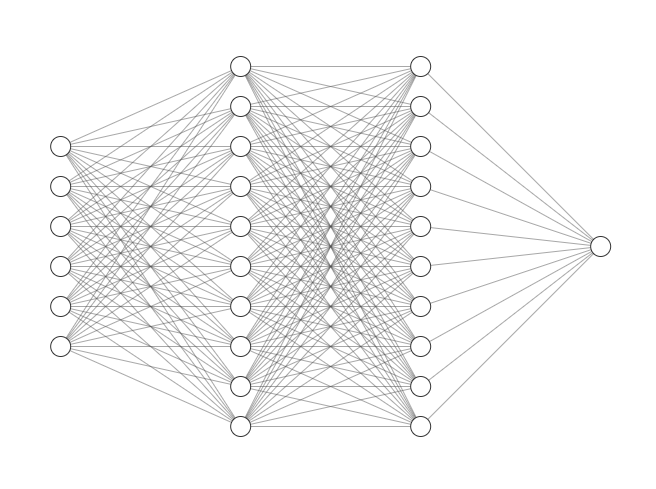
\includegraphics[width=0.9\textwidth]{figs/fcn.png}
    \caption{Przykładowa sieć w pełni połączona}
    \label{fig:fcn}
\end{figure}

Niech \(\bm{L}: \mathbb{R}^{n} \mapsto \mathbb{R}^{m}\) oznacza przekształcenie afiniczne postaci
\[
\bm{L}^\mu(\bm{x}; \bm{W}, \bm{b}) = \bm{b}^\mu + \sum_{\nu=1}^{n} \bm{W}^{\mu\nu}\bm{x}^\nu\,,
\]
gdzie \(\bm{W} \in \mathbb{R}^{m \times n}, \bm{b} \in \mathbb{R}^m\). Dodatkowo przez złożenie
funkcji skalarnej \(a: \mathbb{R} \mapsto \mathbb{R}\) z funkcją \(\bm{L}\) będziemy rozumieć
funkcję \(a \circ \bm{L} : \mathbb{R}^n \mapsto \mathbb{R}^m\)
\[
(a \circ \bm{L})^\mu (\bm{x}) = a\left(\bm{L}^\mu(\bm{x})\right) = a\left(\bm{b}^\mu + \sum_{\nu=1}^{n} \bm{W}^{\mu\nu}\bm{x}^\nu\right)\,.
\]
Sieć w pełni połączona złożona z \(k+2\) warstw o rozmiarach \(n_\text{in}, n_1, \ldots, n_k,
n_\text{out}\) realizuje zatem przekształcenie \(\bm{\phi}: \mathbb{R}^{n_\text{in}} \mapsto
\mathbb{R}^{n_\text{out}}\)
\[
\boxed
{
\bm{\phi}\left(\bm{x}; \left\{(\bm{W}_i, \bm{b}_i)\right\}_{i=1}^{k+1}\right) = \left( \bm{L}_{k+1} \circ a \circ \bm{L}_k \ldots a \circ \bm{L}_2 \circ a \circ \bm{L}_1 \right) (\bm{x}) \,,
}
\]
gdzie \(\bm{L}_i : \mathbb{R}^{n_{i-1}} \mapsto \mathbb{R}^{n_i}\) (przy czym \(n_0 = n_\text{in}\)
i \(n_{k+1} = n_\text{out}\))
\[
\boxed
{
\bm{L}_i^\mu \left(\bm{x}; \bm{W}_i, \bm{b}_i\right) = \bm{b}_i^\mu + \sum_{\nu=1}^{n_{i-1}} \bm{W}_i^{\mu\nu}\bm{x}^\nu\,,
}
\]
\(\bm{W}_i \in \mathbb{R}^{n_i \times n_{i-1}}, \bm{b}_i \in \mathbb{R}^{n_i}\). Okazuje się, iż
taka postać rodziny funkcji parametryzowanych przez wagi i obciążenia \(\bm{W}, \bm{b}\) potrafi
aproksymować niemal dowolną funkcję (\textit{Universal Approximation Theorem}), zatem jest to niemal
uniwersalny aproksymator, który możemy zastosować do wszelkich omawianych wcześniej zagadnień
regresji i klasyfikacji. Zauważmy, iż już wcześniej rozwinęliśmy teorię w sposób dość ogólny
wyprowadzając większość wyników dla pewnej dowolnej funkcji \(\bm{\phi}(\bm{x}; \bm{W})\) i jedynie
na końcu znajdując dokładne rozwiązania dla prostego odwzorowania liniowego \(\bm{W}\bm{x}\) (na
marginesie takie proste odwzorowanie odpowiada płytkiej sieci neuronowej o \(k=0\) warstwach
ukrytych).

\begin{quote}[\textit{Notes, Ch. 4} \cite{prince2023understanding}]
\begin{itemize}
\item \textbf{Deep learning}: It has long been understood that it is possible to build more complex
functions by composing shallow neural networks or developing networks with more than one hidden
layer. Indeed, the term “deep learning” was first used by Dechter (1986). However, interest was
limited due to practical concerns; it was not possible to train such networks well. The modern era
of deep learning was kick-started by startling improvements in image classification reported by
[Alex] Krizhevsky et al. (2012) [AlexNet moment]. This sudden progress was arguably due to the
confluence of four factors: larger training datasets, improved processing power for training, the
use of the ReLU activation function, and the use of stochastic gradient descent.

\item \textbf{Depth efficiency}: Several results show that there are functions that can be realized
by deep networks but not by any shallow network whose capacity is bounded above exponentially. In
other words, it would take an exponentially larger number of units in a shallow network to describe
these functions accurately. This is known as the depth efficiency of neural networks.

\item \textbf{Width efficiency}: Lu et al. (2017) investigate whether there are wide shallow
networks (i.e., shallow networks with lots of hidden units) that cannot be realized by narrow
networks whose depth is not substantially larger. They show that there exist classes of wide,
shallow networks that can only be expressed by narrow networks with polynomial depth. This is known
as the width efficiency of neural networks. This polynomial lower bound on width is less restrictive
than the exponential lower bound on depth, suggesting that depth is more important. Vardi et al.
(2022) subsequently showed that the price for making the width small is only a linear increase in
the network depth for networks with ReLU activations.
\end{itemize}
\end{quote}


% \subsection{Loss functions: MLE, univariate regression, multi-class classification, cross-entropy loss}

% \subsection{Aspekty optymalizacyjne (gradient descent, stochastic gradient descent, momentum, adam)}

% \subsection{Algorytm wstecznej propagacji błędu, automatyczne różniczkowanie}

% \subsection{Regularyzacja i inicjalizacja w sieciach głębokich}

% \subsection{Measuring performance}

% \subsection{Convolutional networks}

% \subsection{Residual networks}

% \subsection{Transformers}


% \section{Natural Language Processing}


% \section{Reinforcement Learning}



\bibliographystyle{plain}
\bibliography{refs} % Entries are in the refs.bib file

\end{document}
